\documentclass{FastFyp}
\usepackage{float} 
\usepackage{longtable}
\usepackage{afterpage}
\begin{document}
\newcommand{\supervisor}{Dr. Zeeshan Ali Khan}
\newcommand{\university}{National University of Computer and Emerging Sciences, Lahore}
\newcommand{\fyptitle}{FASTGlide}
\newcommand{\degree}{BS}
\newcommand{\Studentone}{Asmar Shahid     21L-1754    BS(CS)} 
\newcommand{\Studenttwo}{Abdul Wahab     21L-5291    BS(CS)}
\newcommand{\Studentthree}{Muhammad Saad Sohail     21L-5344    BS(CS)}
\date{\today}
\renewcommand{\contentsname}{Table of Contents}

\makeatletter
    \begin{titlepage}
        
\includegraphics[width=0.2\linewidth]{Figures/nulogo.png}\hfill
        
\includegraphics[width=0.2\linewidth]{Figures/fast.png}\\
        \begin{center} 
            {\large\bfseries \university}\\[7ex]
            
\includegraphics[width=0.4\linewidth]{Figures/fastlogo.png}\\[8ex]
            {\huge \bfseries  \fyptitle }\\[10ex] 
            {\Studentone}\\{\Studenttwo}\\{\Studentthree}\\[4ex] 
            {Supervisor: \supervisor} \\ [10ex]
            {Final Year Project}\\
            {\large \@date}
        \end{center}
    \end{titlepage}    
\makeatother
\frontmatter

\newpage \thispagestyle{empty} \mbox{} \newpage %Aatira

\pagestyle{empty}  %Aatira
\section*{\begin{center}{Anti-Plagiarism Declaration} \end{center}} %Aatira
This is to declare that the above publication was produced under the:
\begin{flushleft}
\bf Title: \fyptitle
\end{flushleft}

is the sole contribution of the author(s), and no part hereof has been reproduced as it is the basis (cut and paste) that can be considered Plagiarism. All referenced parts have been used to argue the idea and cited properly. I/We will be responsible and liable for any consequence if a violation of this declaration is determined.
\\[4ex]
%% FYPTODO add the date and your names here
Date: December 8, 2024

\begin{flushright}
Name: Asmar Shahid
\\[3ex]
Signature: ..........................
\\[6ex]
Name: Abdul Wahab
\\[3ex]
Signature: ..........................
\\[6ex]
Name: Muhammad Saad Sohail
\\[3ex]
Signature: ..........................

\end{flushright} 

\vspace{5 cm} %Aatira
 
\hrule %Aatira

\section*{Author's Declaration}
This states Authors’ declaration that the work presented in the report is their own, and has not been submitted/presented previously to any other institution or organization.
\pagebreak
\section*{Abstract}
The Final Year Project (FYP) is a significant aspect of a student’s degree. It tests whether the
student has successfully learnt the concepts and skills that were taught during the degree
program. It also evaluates the student’s work ethic, technical skills, and domain knowledge.
However, the entire process of registering for the FYP , finding a group, choosing a
supervisor, and completing other requirements is hectic and requires frequent trips to the
university. Supervisors and coordinators also face challenges in managing all their tasks.
FASTGlide aims to assist all those involved in the FYP process by automating and
streamlining the entire process from registration to project completion.
\pagebreak 

\section*{Executive Summary}
The Final Year Project (FYP) stands as a compulsory academic requirement worked towards by students undergoing their final year of undergraduate studies. In computing programs, for instance, students could either develop programs addressing real life problems or explore various advanced computer science areas or work on other goals oriented towards mastering subjects offered in their academic years.

At FAST-NUCES, and like most other universities, the FYP is equally important throughout the period of undergraduate studies. FYP involves several steps including registration, submission of interim project reports and it ends with evaluation. In each of these situations, students, and faculty members including FYP coordinators, have to deal with many issues and administrative problems.

Usually, students experience problems on how to group together without a specific platform for this purpose. They either use their connections or turn to the FYP coordinators asking for help in sending out a mass email to find group members. After groups when formed, other than being challenged by the logistics of finding members, students are also faced with the problem of how to approach a supervisor which often means movement from one teacher’s classroom to another making a shy pitch of the project to each one of them – a resource wasting activity which often leads to several visits.

On the other hand, supervisors get so many emails and see many students who want to be advised on some issues, or to get a decision on submitting a project. Once they agree to be the supervisors of some groups, handling several groups of students becomes a problem. FYP coordinators, who manage the process as a whole, are also equally worse off as they have to deal with updating group information or ensuring the right format is used for every submitted work in a very manual manner.

Through the use of the latest web technologies, our project FASTGlide endeavours to resolve these problems by transforming and improving the Final Year Project Process. FASTGlide plans to reduce the effort of all the parties by reorganizing the processes of forming groups, assigning supervisors, submission of deliverables and their follow ups to make the proceedings more organized and easy.

On the technical side of things, the FASTGlide software development is based on the MERN (MongoDB, Express, React, Node.js) technology stack which enables dynamic and scalable web applications. The front-end is developed using React which makes the interface easy to use by providing a simple interaction with the users, whereas the back-end is developed using Express and Node.js which implements the API and the server-side logic. The database used in this solution is MongoDB which is a NoSQL database that allows for agile development of applications with complex data types such as students, supervisors, and their deliverables.

As part of our research work, we also explored other similar applications like Google Classroom, Basecamp, and MS Teams, among others. While these offer features for project management and team collaboration, none of them was developed primarily to support the FYP process. In contrast, FASTGlide is a solution which takes care of the particular issues that students, supervisors, and coordinators at FAST-NUCES encounter during the FYP cycle.
\pagebreak


\pagestyle{fancy} %Aatira
\tableofcontents

\pagebreak
\listoffigures	% comment this if there are no figures
\addcontentsline{toc}{chapter}{List of Figures}
\pagebreak
\listoftables % comment this if there are no tables
\addcontentsline{toc}{chapter}{List of Tables}

\mainmatter


\chapter{Introduction}
Final Year Project (FYP) is a required academic assessment undertaken by students in their
last year of undergraduate studies. Students studying in computing programs create
applications for real-world problems, research in advanced subjects of computer science, or
work on some other goal with the purpose of demonstrating their proficiency in the subjects
they studied during their degree.

FAST-NUCES, like other universities, also has the FYP requirement for all undergraduate
students. The FYP process begins with registration, consists of submissions of multiple
deliverables, and culminates with the final evaluation. Throughout the process, all the people
involved in it have to undergo a lot of tedious work.

The students have to worry about finding like-minded individuals to form groups with. There
is no channel for them to do so and they have to rely on asking their friends or the FYP
coordinators to send emails to help them find group members. Once this task is done with, the
group members have to find a supervisor for their project. They have to visit the offices of
different teachers multiple times, and have to explain their project idea separately to all of
them.The teachers who take the role of FYP supervisor are disturbed by constant emails and officevisits by students looking for a supervisor. After they have finalized their groups, they find it
hard to keep track of all of them. The FYP coordinators, in particular, have to do a lot of work manually. For example, if any student wishes to change their group details, the coordinators have to manually make the changes. They have to go through every single deliverable to verify that it follows the correct format.

Our project FASTGlide seeks to resolve the above-mentioned issues and modernize the FYP
process through modern web technologies. It will solve the above-mentioned problems and make the process easier.
\section{Purpose of this Document}
The purpose of this document is to outline the various challenges faced in the FYP process and how our application FASTGlide aims to solve those challenges. It clarifies the goals and objectives of our project, as well as the various technologies and strategies we will be using to fulfill those. Throughout this report, we will be discussing the scope of our project, overview of related applications, and the detailed design and functionalities of our application.
\section{Intended Audience}
The document’s intended audience include all the individuals involved in some way 
in the FYP registration and supervision processes. These include the supervisors, coordinators, and students undertaking the FYP. This document will help them understand how making use of this web application can significantly reduce their tedious work and streamline the required processes.
\section{Definitions, Acronyms, and Abbreviations}
Important definitions, acronyms, and abbreviations used in this document are listed below.
\\ \\
\textbf{FYP}: Final Year Project\\
\textbf{UI}: User Interface\\
\textbf{UX}: User Experience\\
\textbf{REST}: Representational State Transfer\\
\textbf{ORM}: Object-Relational Mapping\\
\textbf{CRUD}: Create, Read, Update, Delete\\
\textbf{API}: Application Programming Interface \\
\textbf{AI}: Artificial Intelligence \\
\textbf{SDG}: Sustainable Development Goal\\
\textbf{JWT}: JSON Web Token\\
\textbf{RBAC}: Role Based Access Control
\section{Conclusion}
The first chapter of this report gives an introduction to FASTGlide, its intended audience, and the multiple terms, acronyms, and abbreviations used throughout the whole report. The second chapter will clarify the vision and scope of our project, as well as any business oppurtunities alongwith the stakeholders’ details. The goals and objectives of our project are also clearly defined. The third chapter involves thorough research of related applications in the market. The fourth chapter outlines the functionalities, requirements, and use cases of FASTGlide. The fifth and last chapter elaborates on the design and architecture of the application and illustrates it with multiple diagrams.
\chapter{Project Vision}
The proposed solution of FASTGlide is built upon the observation that the Final Year Project (FYP) system at FAST-NUCES is cumbersome and time-consuming. The goal of the platform is to practically eliminate all the intermediaries and make all stages starting from registration and ending up with the completion of the FYP as smooth as possible for students, their supervisors and FYP coordinators. To achieve its stated goals, FASTGlide seeks to utilize current-generation web technologies and artificial intelligence in enhancing collaboration between the various entities.
\section{Problem Domain Overview}
There are some problems existing in the current FYP process at FAST–NUCES. Some challenges students experience include; formation of working groups, identification of supervisors and assurance of compliance with production standards. Supervisors can fail to monitor the progress of several projects and interruptions from students. On the other hand, FYP coordinators find themselves dealing with several manual processes, including checking of deliverables and making group alterations which is inefficient and can be very incorrect.
\section{Problem Statement}
The FYP process as it is practiced at FAST-NUCES is somewhat lengthy and convoluted at the moment. The challenges range from group formation, identification of supervisors and on the other side the supervisors struggle with managing different projects. FYP coordinators receive the burden of entering their own data, verification of students’ deliverables and updating the group information. This calls for an automated system that will handle the entire process.
\section{Problem Elaboration}
Currently, there exists no formal system that can help students to find group members. When the groups are formed students are forced to go and explain their ideas to the supervisors severally. As a result, for supervisors it results in confusion and time management issues. Coordinators are responsible for manually entering group details adjustments and changes to formats of the submissions, thus contributing to an inefficient and error-prone procedure. These inefficiencies harm everyone involved, which is why they require an improved approach.
\section{Goals and Objectives}
The goal of our project is to create an automated workflow for FYP submission in FAST. We
aim to achieve the following objectives:
\begin{itemize}
    \item To help the students undertaking FYP in finding groups and relevant supervisor for
their project
   \item To assist the supervisors in managing the projects they are supervising and monitor
their progress.
   \item To automate checking of deliverables and other tasks which are currently performed
manually by FYP coordinators
\end{itemize}
\section{Project Scope}
FASTGlide will be a web-based application, making it accessible across platforms. The project aims to benefit final-year students, supervisors, and the FYP committee at FAST-NUCES School of Computing. It will assist students in forming project groups, supervisors in overseeing multiple projects efficiently, and coordinators in automating the verification of deliverables and other repetitive tasks. Through this system, the FYP process will be more organized, reducing the workload for all involved parties and enhancing the overall experience.
\section{Sustainable Development Goal (SDG)}
FASTGlide is targeting the Sustainable Development Goal (SDG) of Quality Education. FASTGlide aims at enhancing the efficiency and accessibility of the process of Final Year Project (FYP) for students. It eases the load of managing and coordinating interactions among students, supervisors, and administrators, ensuring smooth education processes. Easy interaction, receiving and giving constructive criticism, and tracking the progress of the project in this case FASTGlide helps to eliminate impediments to access quality learning and enhances creativity in managing academic projects and initiatives.
\begin{figure} [H]
    \centering

\includegraphics[width=0.25\textwidth, height=0.15\textheight]{Figures/Picture1}
    \caption{Quality Education}
    \label{fig:1}
\end{figure}
\section{Constraints}
Every one of FASTGlide’s potentialities mentioned earlier has its drawbacks too. First, there are budgetary limits that may slow down project development and limiting project scope as with insufficient money it may be difficult to acquire resources. Resources may be some constraints to the development of the project, especially when it comes to the technical side of the platform and making the same available on all devices. It is possible that there may be other hurdles resulting from internal governing policies, such as regulation of academic administration. Lastly, it is important to emphasize the need of users - it may take time to convince students, supervisors, and coordinators to shift from manual work to computerized systems.
\section{Business Opportunity}
Through the boosting of project inefficiencies, FASTGlide brings a very lucrative market opportunity relating to the FYP process. The system has potential for wider usage in other universities as it provides them with a good project management system. Besides, FASTGlide is such a well-known system that it aims offering additional services, including but not limited to supervisors’ performance analytics and students’ AI help in finding project ideas which creates possibilities for launching new subscription-based or licensing models of the platform in the future.
\section{Stakeholders Description/ User Characteristics}
FASTGlide is participative in a number of relevant stakeholders who contribute significantly to the Final Year Project (FYP) process and these are students, supervisors and FYP coordinators. The system, the role played by each individual as well as guidelines on how each of them interacts with the system differs quite a lot.
\subsection{Stakeholders Summary}
\subsubsection{Students}
Students remain the first and frequent users of the FASTGlide platform. They are mostly in their undergraduate final year and have to fulfill the FYP requirement for graduation. In theirs, they seek to meet and recruit persons for project groups, a suitable project supervisor and timely submission of project deliverables. At present, students are forced to use informal groups and contacts or the help of the coordinators to join groups. This procedure, FASTGlide provides as an opportunity to search for future group members through targeted interest or skills. In addition, students will have a single application where they will perform all actions related to the FYP coordination – submitting project ideas, project deliverables or feedback requests and tracking supervisor’s comments.
\subsubsection{Supervisors (Faculty Members)}
The involvement of faculty members as project supervisors is necessary for steering students throughout the FYP process. Supervisors have issues in terms such as trying to manage student groups that are in the same level and evaluating the extent of their work and giving the necessary comments. In the case of FASTGlide, supervisors will have a dashboard that will ease the management of all the groups that have been assigned to them. They will manage deliverables, and even track the milestones that have been achieved, and interact with students easily. Further, the system will assist the supervisors in time management by cutting down on repeated visits to the office and individual emails from students.
\subsubsection{FYP Coordinators} 
The activities of the students are from the time when the students are registered to the time the projects are physically completed and that is the FYP coordinators’ duty. Nowadays, coordinators are greatly overburdened because paperwork that is supposed to be automated is still performed manually. For instance, capturing changes in the group members, confirming whether the task was completed, and making sure that the work meets university standards; all these officials still perform them manually. Majority of these activities will be handled by FASTGlide and therefore the workload for the coordinators is bound to reduce. The site will give guidance on the correct procedures for submitting group documents and checking the final submission. This automation will lower the number of routine tasks done and also help to keep the FYP process on track.
\subsection{Key High-Level Goals and Problems of Stakeholders}
Different stakeholder groups have different goals and challenges, which FASTGlide will endeavor to understand and tackle:

\subsubsection{Students}
\textbf{Goals:} Create a central web platform that makes the process of finding groups, getting a supervisor, and submitting the project deliverables easier.
\\
\textbf{Problems:} The current situation is rather inefficient and takes quite a lot of time. It forces students to come to university several times and manually communicate with students and faculty.

\subsubsection{Supervisors (Faculty Members)}
\textbf{Goals:} Enhancing their ability to multitask on projects, monitor student activities, and return comments on time
\\
\textbf{Problems:} Emailing back and forth or making a trip to the office is an extremely inefficient system which has room for errors leading to missed appointments or deadlines.

\subsubsection{FYP Coordinators} 
\textbf{Goals:} Replace these manual processes, for example, verification of deliverables, making updates to group databases, as well as report writing by employing FYP system.
\\
\textbf{Problems:} Inconvenience posed by manual handling of task processes, risk of underperformance due to human factor.

\chapter{Literature Review / Related Work}
In the domain of educational technology, there are a number of applications that are designed to make the process of learning, working together and managing projects more efficient. This section covers a number of tools that are already available in the academic or professional use and focuses on their advantages as well as the relation of these tools to the concept of FASTGlide, which is intended to revolutionize and improve the Final Year Project (FYP) process.
\section{Definitions, Acronyms, and Abbreviations}
Important definitions, acronyms, and abbreviations used in this section are listed below.\\ \\
\textbf{FYP}: Final Year Project\\
\textbf{AI}: Artificial Intelligence\\
\textbf{LMS}: Learning Management System
\section{Detailed Literature Review}
\subsection{Google Classroom}
In educational institutions, Google Classroom \cite{ref:classroom} is an online course management system that allows making coursework, assignments, and communication easier. It also enables educators to set up classes, send the coursework to students, mark it and interact among students and instructors. It is a Google workspace integrated system; it provides collaborative working business tools such as Docs, Sheets, and Slides for group work, plus a cloud net storage system called Google Drive.
\subsubsection{Critical analysis of the related work}
There is no doubt that google classroom can help one manage their assignments as well as submit them, however it does not have the adequate tools to support the intricacies involved with undertaking a final year project. This general purpose features, although are practical do not provide the necessary essential elements of project management such as the tracking of progress, management of milestones achievements, and faculty and students communication that is needed for projects like the FYPs. It also lacks provision for advanced analytics and an effective proposal submission and approval process with well-defined hierarchies, which in fact are central in achieving the objectives of FASTGlide.
\subsubsection{Relationship to the proposed related work}
Google Classroom and FASTGlide share the common objective of easing the students’ academic burden, however, Google Classroom is more course management oriented. FASTGlide on the other hand is designed for the FYP processes and provides functionalities like milestone management, communication between supervisors and students, and automating proposal processes making it suitable for the academic project management cycle.
\subsection{Gradescope}
Gradescope \cite{ref:gradescope} is a system that assists in marking quizzes and tests, tailored towards enhancing the efficiency of the grading processes for the instructors. It incorporates tools for AI grading, assessing using a grading rubric and LMS integration.
\subsubsection{Critical analysis of the related work}
For large classes or courses with complex grading tasks, Gradescope shines in grading speed. The tool, however, does not reach to areas such as coordination of students and faculties in relation to projects in real time, which is a very crucial aspect in an FYP. Furthermore, its main focus is on evaluation processes rather than the management and automation of the project life cycle.
\subsubsection{Relationship to the proposed related work}
As much as Gradescope concentrates on automating the grading process, FASTGlide goes a step further and integrates proposal focusing on the project management aspect of a project in its proposal, milestone reporting, and collaboration. There is a broader range of tasks performed in FASTGlide other than grading which includes project performance measurements at various levels which are not covered by Gradescope.
\subsection{Microsoft Teams}
Microsoft Teams \cite{ref:teams} is a versatile platform for communication, enabling instant messaging, video conferencing, data storage as well as integration of other applications. It is often referred to as a team working space within educational institutions and workplaces, with its ability to support team interactions and sharing of files and information supported by other activities such as management of tasks and scheduling.
\subsubsection{Critical analysis of the related work}
Despite the fact that Teams allows video conferences, real time chats and exchange of documents, it does not have any feature designated for management of a final year project. It does not have a well-defined submission process for the project deliverables. It does not have any mechanism for tracking project milestones, nor does it assign any task to a supervisor or a student for that matter. While it helps in collaborative work, it does not address the education processes in final year projects that FASTGlide is to address.
\subsubsection{Relationship to the proposed related work}
There are effective collaboration tools in Microsoft Teams application but FASTGlide has its focus on automating tasks that are relevant to FYPs. Approval processes and specialized workflows of FASTGlide are meant to enhance the particular project management functions that an academic institution has, for which Teams lacks inbuilt functionality.
\subsection{Basecamp}
Basecamp \cite{ref:basecamp} is an application that helps teams in managing projects by breaking down tasks, allocating them to the relevant persons, and monitoring the developments. Such facilities include to-do lists, message boards, schedules and file sharing in order to help all the members of the team to work as one.
\subsubsection{Critical analysis of the related work}
Relatively, Basecamp is very good in generic project management but it does not have particular academic functionalities that are crucial for FYPs such as communication with the professors or even grading. Moreover, it does not have the management and statistics features that are necessary for proper control of educational projects.
\subsubsection{Relationship to the proposed related work}
Basecamp’s project management characteristics closely fit systems in the project-tracking category of FASTGlide. Nevertheless, FASTGlide comes with additional academic features such as grading systems, activity tracking systems, and faculty systems that simplify endorsements but Basecamp does not include such modules.
\subsection{Moodle}
Moodle \cite{ref:moodle} is a popular open-source LMS learning platform that is mostly utilized by educational institutions. It helps teachers to build online course, conduct assessments, and monitor the academic performance of students.
\subsubsection{Critical analysis of the related work}
Moodle has robust capacity for online learning and assessment. However, it does not in any way support the work processes of the final year programme (FYP). It is able to run courses, but there are no means of automating the project acceptance or the requisition for feedback which are core to FYPs. Moreover, the elements of the system are quite complicated as well as its use for assisting the specific requirements of a final-year student.
\subsubsection{Relationship to the proposed related work}
Moodle covers a wide spectrum of online education, while FASTGlide strives to enhance only the FYP flow. FASTGlide’s benefits are appreciated in the components which are aimed at controlling the processes of FYPs and are not provided fully through a wide range of Moodel’s LMS offered solutions.
\subsection{Canvas}
Canvas \cite{ref:canvas}, like many others, is yet another learning management system that is used in most educational institutions. It is mostly course management oriented and provides support in organizing assignments, grades and feedback for students.
\subsubsection{Critical analysis of the related work}
Canvas, like many others, is yet another learning management system that is used in most educational institutions. It is mostly course management oriented and provides support in organizing assignments, grades and feedback for students.
\subsubsection{Relationship to the proposed related work}
Canvas is adequate in terms of managing academic activities in general. Canvas does not possess the tools that deal with the intricacies of final year projects, hence FASTGlide is more configurable in that that it provides tools for final year project activities.
\subsection{Sakai}
Sakai \cite{ref:sakai} is an open source learning management system is adopted by many educational institutes for online courses, grading of students, and students’ interactions. It accentuates adaptability and personalization to different learning environments.
\subsubsection{Critical analysis of the related work}
Although Sakai’s design allows for an easy incorporation of many factors, it may have to be extensively redesiged in order to effectively manage projects such as students FYPs. Basic workflow communications such as project and milestone approvals, FYP faculty to student communications tools, and other controls as required in an FYP, are not provided.
\subsubsection{Relationship to the proposed related work}
FASTGlide offers better tailored academic project management solution that centers around FYP specifications. Sakai’s broader course management functionalities present good chances of enhancing the efficacy of managing processes with final year students and their supervising professors but fail to meet the general requirements of the users.
\subsection{Blackboard}
Blackboard \cite{ref:blackboard} is one of the most popular learning management systems available as it facilitates the management of courses, assignments, and interaction with students for educational institutions. It enables grading, assessment, and interaction between students and educators.
\subsubsection{Critical analysis of the related work}
Blackboard has provided an all-encompassing academic management suite of tools however this has not been designed for workflows that are strictly project based such as FYPs. Further it lacks automated process to facilitate project completion, monitoring of milestones achieved and performance statistics which are critical management activity of academic projects.
\subsubsection{Relationship to the proposed related work}
The LMS functions of the Blackboard overlap with the functions of many other systems including that of FASTGlide project management system, which is specifically designed for FYPs. FASTGlide provides a solution to the functionality of Blackboard by allowing management of final year projects which have their own complexities in a simplified manner.
\subsection{Edmodo}
Edmodo \cite{ref:edmodo} is a learning management system (LMS) that promotes interaction between students and teachers. It is a platform where educators can prepare their assignments, quizzes, and polls, while allowing students to engage, turn in their work, and get resources for study. The instructor can also grade the work and carry out assessments of each student’s performance based on predefined metrics.
\subsubsection{Critical analysis of the related work}
Although Edmodo is a satisfactory general purpose classroom engagement tool that incorporates such features as submitting assignments and communicating with learners, it does not have the necessary features to manage final year projects (FYPs) for colleges and universities. It does not allow for tracking of milestones, facilitate an approval workflow process automatically, or even provide any form of analytics as far as academic projects focused on FYP’s are concerned. More attention is paid on operating within manageable units of a day or two in class than organizing and coordinating work over a couple of weeks or months.
\subsubsection{Relationship to the proposed related work}
Edmodo may allow submission of assignments and interaction with the students but FASTGlide aims to make the FYP process quicker and more efficient. There are specific offerings tailored for FYP management like tracking of proposal submissions, controlling of milestones and student’s supervisors which makes this system better fitted for a very particular purpose unlike Edomo where the focus is on management of classroom activities.
\subsection{Brightspace by D2L}
Brightspace \cite{ref:brightspace} is a comprehensive LMS for higher learning institution with content management, quizzes, grading, and analytics, among others. It endorses blended learning and has course management, learning progress, and student interaction tools.
\subsubsection{Critical analysis of the related work}
 Brightspace has a massive potential in terms of coursework and student performance management but focuses mainly on general systems and does not suit the precise management of the FYP. Further, it does not have features such as automated systems for FYP approvals, timelines for the completion of project phases, and various supervisor-to-student interactions focused on the academic nature of projects. Also, although it is true that Brightspace does have analytic aspects with regards to course performance, it does not have any of the pertinent FYP analytics.
\subsubsection{Relationship to the proposed related work}
While Brightspace has got all the essential components of an LMS which enhances academic management systems, FASTGlide focuses solely on FYPs. FYP-specific project submission processes for example, supervisor assessment and milestone tracking are features that are unavailable in Brightspace but are present in the software. The design of FASTGlide captures this unique need of final year students and their supervisors hence it is more preferred and focused on the management of final year projects.
\pagebreak
\section{Literature Review Summary Table}

\begin{longtable}{|p{2.5cm}|p{2.5cm}|p{4cm}|p{5cm}|}
\caption{Summary of Related Work} \\
\hline
\textbf{Application} & \textbf{Features} & \textbf{Relevance} & \textbf{Limitations} \\
\hline
\endfirsthead

\hline
\textbf{Application} & \textbf{Features} & \textbf{Relevance} & \textbf{Limitations} \\
\hline
\endhead

\hline
\multicolumn{4}{r}{\textit{Continued on the next page}} \\
\hline
\endfoot

\hline
\endlastfoot

Google Classroom \cite{ref:classroom} & User-friendly interface for managing coursework, assignments, and class communications & Streamlines the process of class management, enabling efficient communication and assignment distribution among students and instructors & Lacks specialized tools for tracking progress and managing the complexities of Final Year Projects (FYP), which may hinder effective project management \\
\hline
Gradescope \cite{ref:gradescope} & AI-assisted grading & Streamlines grading, allowing instructors to evaluate large numbers of assignments efficiently & Focuses on grading, not project management or collaboration needed for FYPs. \\
\hline
Microsoft Teams \cite{ref:teams} & Comprehensive collaboration platform & Enhances communication and teamwork among students and faculty & Lacks FYP-specific features like milestone tracking and project oversight. \\
\hline
Basecamp \cite{ref:basecamp} & Project management tool & Provides a structured approach to managing tasks and projects & Does not cater to the academic environment, lacking educational compliance features. \\
\hline
Moodle \cite{ref:moodle} & Open-source learning management system & Facilitates course creation and student tracking & Lacks specific FYP workflows and automated processes for project submissions. \\
\hline
Canvas \cite{ref:canvas} & User-friendly course management tools & Supports efficient management of assignments and grading & Does not specifically address the unique requirements of FYPs or their management. \\
\hline
Sakai \cite{ref:sakai} & Flexible course management platform & Customizable for different academic needs & Requires significant setup time for customization to meet FYP requirements. \\
\hline
Blackboard \cite{ref:blackboard} & Comprehensive academic management tools & Streamlines course administration & Lacks dedicated project management features for Final Year Projects. \\
\hline
Edmodo \cite{ref:edmodo} & Classroom management tools & Enhances classroom interaction and communication & Focuses on day-to-day activities rather than long-term project management. \\
\hline
Brightspace \cite{ref:brightspace} & Advanced learning management system & Offers robust analytics and course management features & Lacks dedicated FYP management capabilities and detailed supervisor-student interaction tools. \\
\hline

\end{longtable}

\section{Conclusion}
The previous chapters examine the usage of diverse computer software within the academic context, concentrating mainly on the organization of the coursework, the interaction between students and instructors, as well as the evaluation of the students’ achievements. Google Classroom \cite{ref:classroom} and Microsoft Teams \cite{ref:teams} provide users with features that facilitate the teaching and the collaborative aspects of the courses, however, they usually do not include the tools that are needed for the successful FYP management. There are such applications as Gradescope \cite{ref:gradescope} or Moodle \cite{ref:moodle} that simplify the grading process and organization of the course but do not help with the specific aspects of the FYP workflow. Furthermore, solutions such as Blackboard \cite{ref:blackboard} and Canvas \cite{ref:canvas} assist in the promotion of academic activities coordination however, they lack project control and task scheduling features that are fundamental to FYPs. From this analysis, it is evident that there is a requirement for such a solution, which covers the limitations of existing ones at the same time improving the experience of all participants during the FYP process for instance students, supervisors and coordinators.
 
\chapter{Software Requirement Specifications}
This chapter highlights important features of the projects. It also includes functional and non-
functional requirement of the project, defines database design and risk analysis involves in the
project.
\section{List of Features}
The system will support the following core features:
\begin{itemize}
    \item Allow students to search for FYP group members.
    \item Notify students about FYP group requests.
    \item Enable students to search for FYP supervisors.
    \item Facilitate online FYP registration.
    \item Enable communication between students and their group members, as well as supervisors.
    \item Allow students to schedule meetings (online or physical) with their supervisor.
    \item Enable students to submit their final deliverable for format verification.
    \item Notify supervisors of FYP registration requests.
    \item Allow supervisors to post FYP project ideas.
    \item Notify supervisors of meeting requests.
    \item Facilitate communication between supervisors and FYP groups.
    \item Allow Coordinators to view the deliverables submissions.
\end{itemize}
\section{Functional Requirements}

The functional requirements fully describe the external behavior of the system. Each functionality is identified and briefly described below, along with the respective users.

\subsection{Functional Requirements for Students}
The system will allow students to:
\begin{itemize}
    \item \textbf{Log in to the FYP portal}: Students will be able to securely log in to access the portal.
    \item \textbf{Complete their profile with relevant information}: Students can update their profile with essential details, including academic and personal information.
    \item \textbf{View project ideas posted by supervisors}: Students can browse and view FYP project ideas posted by different supervisors.
    \item \textbf{Connect with other students to form FYP groups}: The system allows students to find and connect with peers to form FYP groups.
    \item \textbf{Reach out to supervisors regarding FYP projects}: Students can communicate with supervisors to discuss project ideas and potential collaboration.
    \item \textbf{Register their FYP project}: Students can officially register their FYP project through the portal.
    \item \textbf{View FYP registration details}: Registered students can view the details of their FYP registration.
    \item \textbf{Communicate with their FYP group members}: A communication feature allows students to stay connected with their group members.
    \item \textbf{Schedule meetings with their supervisor}: The system enables students to schedule either online or physical meetings with their supervisor.
    \item \textbf{Submit the FYP deliverables}: Students can upload their final FYP deliverables for review and approval.
\end{itemize}

\subsection{Functional Requirements for Supervisors}
The system will allow supervisors to:
\begin{itemize}
    \item \textbf{Post FYP project ideas}: Supervisors can post FYP project ideas for students to review and consider.
    \item \textbf{View student requests to join an FYP project}: Supervisors can see requests from students interested in joining their project.
    \item \textbf{Accept or reject student requests}: Supervisors have the ability to approve or decline student requests to join their project.
    \item \textbf{Register FYP groups}: Supervisors can formally register FYP groups within the system.
    \item \textbf{Communicate with the members of the FYP groups}: Supervisors can directly communicate with the FYP group members.
\end{itemize}

\subsection{Functional Requirements for Coordinators}
The system will allow coordinators to:
\begin{itemize}
    \item \textbf{View the deliverables submitted by the student}: Coordinators can review the final deliverables submitted by students.
    \item \textbf{Set the deadlines for the deliverables}: Coordinators can establish and manage deadlines for the submission of FYP deliverables.
    \item \textbf{Post any announcement for the students}: Coordinators can publish announcements and updates for students through the system.
\end{itemize}

\subsection{Functional Requirements of the System}
The system will:
\begin{itemize}
    \item \textbf{Recommend potential group members to students for FYP}: The system will suggest possible group members for students based on relevant criteria.
    \item \textbf{Suggest suitable supervisors for students}: Based on project interests, the system will recommend appropriate supervisors to students.
    \item \textbf{Handle FYP registration}: The system will manage the registration process for FYP projects, ensuring accurate tracking of project registrations.
    \item \textbf{Notify both students and supervisors about updates and requests}: The system will send notifications to keep both students and supervisors updated on requests and changes.
    \item \textbf{Facilitate meeting scheduling between students and supervisors}: The system will assist in scheduling meetings between students and their supervisors.
    \item \textbf{Verify the formatting of the submitted final deliverables}: The system will check the format of submitted deliverables to ensure they meet the required standards.
\end{itemize}

\section{Non-Functional Requirements}

This section describes the non-functional requirements, including performance, reliability, usability, security, scalability, maintainability, and portability of the system.

\subsection{Performance}
\begin{itemize}
    \item The system should allow users to access the FYP portal and load pages within 5-10 seconds under normal conditions.
    \item It should be able to handle concurrent usage by a realistic number of users (students, supervisors) without noticeable lag or degradation in performance.
\end{itemize}

\subsection{Reliability}
\begin{itemize}
    \item The system should aim for 99\% uptime, ensuring high availability throughout the FYP submission period.
    \item Backup and recovery mechanisms should be in place to minimize data loss in case of system failure.
\end{itemize}

\subsection{Usability}
\begin{itemize}
    \item The system will provide an intuitive, user-friendly interface that allows users to navigate and use all core functionalities (FYP registration, group formation, communication, etc.) without extensive training.
    \item The interface should be self-explanatory, enabling users to complete tasks in a few minutes.
    \item It should also be accessible on a wide range of devices, such as laptops, tablets, and smartphones.
\end{itemize}

\subsection{Security}
\begin{itemize}
    \item User data such as profile information, FYP details, and communications must be securely stored, ensuring confidentiality and privacy.
    \item The system should implement secure authentication and authorization mechanisms to prevent unauthorized access to sensitive information.
    \item All data exchanges, especially during communication and registration, should be encrypted (e.g., using SSL/TLS).
\end{itemize}

\subsection{Scalability}
\begin{itemize}
    \item The system should be scalable to support an increasing number of students and supervisors over time without performance degradation.
    \item It should be easy to upgrade or modify features to accommodate future requirements, such as adding new types of FYP projects or expanding to other departments.
\end{itemize}

\subsection{Maintainability}
\begin{itemize}
    \item The system will follow modular design principles, making it easier to maintain and update.
    \item The code should be well-documented to allow future developers to easily understand and make modifications as needed.
\end{itemize}

\subsection{Portability}
\begin{itemize}
    \item The system should be designed to run on various operating systems and browsers that support JavaScript and modern web technologies.
    \item It should be deployable on different environments (on-premise or cloud-based) without significant changes.
\end{itemize}

\section{Assumptions}

The following assumptions have been made for the system specification:

\begin{itemize}
    \item The end users have access to a browser with JavaScript compatibility installed on their devices.
    \item A stable internet connection is available for all users to interact with the system.
    \item Users are expected to have a basic understanding of common website functionalities, such as navigation and form submission.
\end{itemize}
\pagebreak
\section{Use Cases}
This section lists relevant use cases that represent central functionalities of our system encompassing all stakeholders.\\

\begin{longtable}{|lllll|}
\caption{Login Process Details} \label{tab:2.1} \\ \hline
\multicolumn{2}{|l|}{\textbf{Name}} &
  \multicolumn{3}{l|}{Login} \\ \hline
\multicolumn{2}{|l|}{\textbf{Actors}} &
  \multicolumn{3}{l|}{Students, Teachers} \\ \hline
\multicolumn{2}{|l|}{\textbf{Summary}} &
  \multicolumn{3}{l|}{\begin{tabular}[c]{@{}l@{}}The user shall provide their email and password on the login form,\\ and after successful verification, redirect the user to the home page.\end{tabular}} \\ \hline
\multicolumn{2}{|l|}{\textbf{Pre-Conditions}} &
  \multicolumn{3}{l|}{\begin{tabular}[c]{@{}l@{}}The user must be in the database records, either added by any of the\\ authorized users or added manually by a developer.\\ The user must not be logged in.\end{tabular}} \\ \hline
\multicolumn{2}{|l|}{\textbf{Post-Conditions}} &
  \multicolumn{3}{l|}{\begin{tabular}[c]{@{}l@{}}The user’s session is successfully established and shall be \\ redirected to the home page.\end{tabular}} \\ \hline
\multicolumn{2}{|l|}{\textbf{\begin{tabular}[c]{@{}l@{}}Special\\ Requirements\end{tabular}}} &
  \multicolumn{3}{l|}{None} \\ \hline
\multicolumn{5}{|c|}{\textbf{Basic Flow}} \\ \hline
\multicolumn{3}{|c|}{\textbf{Actor Action}} &
  \multicolumn{2}{c|}{\textbf{System Response}} \\ \hline
\endfirsthead % The first header for the table
\hline
\multicolumn{3}{|c|}{\textbf{Actor Action}} &
  \multicolumn{2}{c|}{\textbf{System Response}} \\ \hline
\endhead % The header for all subsequent pages
\multicolumn{1}{|l|}{1} &
  \multicolumn{2}{l|}{The user opens the login page.} &
  \multicolumn{1}{l|}{2} &
  \begin{tabular}[c]{@{}l@{}}The login page is displayed asking for \\ email and password.\end{tabular} \\ \hline
\multicolumn{1}{|l|}{2} &
  \multicolumn{2}{l|}{The user enters valid email and password.} &
  \multicolumn{1}{l|}{4} &
  \begin{tabular}[c]{@{}l@{}}The system verifies the email and password,\\ establishes a session for the user, and\\ redirects the user to the home page.\end{tabular} \\ \hline
\multicolumn{5}{|c|}{\textbf{Alternative Flow}} \\ \hline
\multicolumn{1}{|l|}{3} &
  \multicolumn{2}{l|}{The user enters invalid email or password.} &
  \multicolumn{1}{l|}{4-A} &
  \begin{tabular}[c]{@{}l@{}}The system responds with an error\\ message: Incorrect email or password entered.\end{tabular} \\ \hline
\end{longtable}

\begin{longtable}{|lllll|}
\caption{Logout Process Details} \label{tab:2.2} \\ \hline
\multicolumn{2}{|l|}{\textbf{Name}} &
  \multicolumn{3}{l|}{Logout} \\ \hline
\multicolumn{2}{|l|}{\textbf{Actors}} &
  \multicolumn{3}{l|}{Students, Teachers} \\ \hline
\multicolumn{2}{|l|}{\textbf{Summary}} &
  \multicolumn{3}{l|}{\begin{tabular}[c]{@{}l@{}}The user shall click on the "Logout" button and will be \\ redirected to the login page.\end{tabular}} \\ \hline
\multicolumn{2}{|l|}{\textbf{Pre-Conditions}} &
  \multicolumn{3}{l|}{The user must be logged in.} \\ \hline
\multicolumn{2}{|l|}{\textbf{Post-Conditions}} &
  \multicolumn{3}{l|}{\begin{tabular}[c]{@{}l@{}}The user's session is successfully ended and \\ the user is redirected to the login page.\end{tabular}} \\ \hline
\multicolumn{2}{|l|}{\textbf{Special Requirements}} &
  \multicolumn{3}{l|}{None} \\ \hline
\multicolumn{5}{|c|}{\textbf{Basic Flow}} \\ \hline
\multicolumn{3}{|c|}{\textbf{Actor Action}} &
  \multicolumn{2}{c|}{\textbf{System Response}} \\ \hline
\endfirsthead % First page header
\hline
\multicolumn{3}{|c|}{\textbf{Actor Action}} &
  \multicolumn{2}{c|}{\textbf{System Response}} \\ \hline
\endhead % Header for subsequent pages

\multicolumn{1}{|l|}{1} &
  \multicolumn{2}{l|}{The user clicks on the "Logout" button.} &
  \multicolumn{1}{l|}{2} &
  \begin{tabular}[c]{@{}l@{}}The system terminates the user’s session and \\ redirects the user to the login page.\end{tabular} \\ \hline
\multicolumn{5}{|c|}{\textbf{Alternate Flow}} \\ \hline
\multicolumn{5}{|l|}{No Alternate Flow} \\ \hline
\end{longtable}



\begin{longtable}{|lllll|}
\caption{Add FYP Post Description Process} \label{tab:2.3} \\ \hline
\multicolumn{2}{|l|}{\textbf{Name}} &
  \multicolumn{3}{l|}{Add FYP Post Description} \\ \hline
\multicolumn{2}{|l|}{\textbf{Actors}} &
  \multicolumn{3}{l|}{Teachers} \\ \hline
\multicolumn{2}{|l|}{\textbf{Summary}} &
  \multicolumn{3}{l|}{\begin{tabular}[c]{@{}l@{}}The user shall click on the "Add Post" button and a pop-up will \\ appear asking for the details of the post.\end{tabular}} \\ \hline
\multicolumn{2}{|l|}{\textbf{Pre-Conditions}} &
  \multicolumn{3}{l|}{The user must be logged in.} \\ \hline
\multicolumn{2}{|l|}{\textbf{Post-Conditions}} &
  \multicolumn{3}{l|}{The new FYP post description is stored in the database.} \\ \hline
\multicolumn{2}{|l|}{\textbf{Special Requirements}} &
  \multicolumn{3}{l|}{None} \\ \hline
\multicolumn{5}{|c|}{\textbf{Basic Flow}} \\ \hline
\multicolumn{3}{|c|}{\textbf{Actor Action}} &
  \multicolumn{2}{c|}{\textbf{System Response}} \\ \hline
\endfirsthead % Header for the first page
\hline
\multicolumn{3}{|c|}{\textbf{Actor Action}} &
  \multicolumn{2}{c|}{\textbf{System Response}} \\ \hline
\endhead % Header for subsequent pages

\multicolumn{1}{|l|}{1} &
  \multicolumn{2}{l|}{The user clicks on the "Add Post" button.} &
  \multicolumn{1}{l|}{2} &
  \begin{tabular}[c]{@{}l@{}}The "Add New Post Description" \\ popup is displayed.\end{tabular} \\ \hline
\multicolumn{1}{|l|}{2} &
  \multicolumn{2}{l|}{The user fills out the necessary fields.} &
  \multicolumn{1}{l|}{3} &
  \begin{tabular}[c]{@{}l@{}}The system validates the entered data.\end{tabular} \\ \hline
\multicolumn{1}{|l|}{3} &
  \multicolumn{2}{l|}{The user clicks the "Post" button.} &
  \multicolumn{1}{l|}{4} &
  \begin{tabular}[c]{@{}l@{}}The system stores the new FYP post \\ description in the database and confirms \\ the successful addition.\end{tabular} \\ \hline
\multicolumn{5}{|c|}{\textbf{Alternate Flow}} \\ \hline
\multicolumn{1}{|l|}{2a} &
  \multicolumn{2}{l|}{The user enters invalid data.} &
  \multicolumn{1}{l|}{4-A} &
  \begin{tabular}[c]{@{}l@{}}The system responds with an error message: \\ Incorrect data entered.\end{tabular} \\ \hline
\end{longtable}

\begin{longtable}{|lllll|}
\caption{Analyzing Process} \label{tab:delete-fyp-post} \\ \hline
\multicolumn{2}{|l|}{\textbf{Name}} &
  \multicolumn{3}{l|}{Analyzing Process} \\ \hline
\multicolumn{2}{|l|}{\textbf{Actors}} &
  \multicolumn{3}{l|}{Students} \\ \hline
\multicolumn{2}{|l|}{\textbf{Summary}} &
  \multicolumn{3}{l|}{The User selects the document for running the analyzing process.} \\ \hline
\multicolumn{2}{|l|}{\textbf{Pre-Conditions}} &
  \multicolumn{3}{l|}{The user must be already logged in.} \\ \hline
\multicolumn{2}{|l|}{\textbf{Post-Conditions}} &
  \multicolumn{3}{l|}{The uploaded document feedback is displayed on the screen} \\ \hline
\multicolumn{2}{|l|}{\textbf{Special Requirements}} &
  \multicolumn{3}{l|}{None} \\ \hline
\multicolumn{5}{|c|}{\textbf{Basic Flow}} \\ \hline
\multicolumn{3}{|c|}{\textbf{Actor Action}} &
  \multicolumn{2}{c|}{\textbf{System Response}} \\ \hline
\endfirsthead % Header for the first page
\hline
\multicolumn{3}{|c|}{\textbf{Actor Action}} &
  \multicolumn{2}{c|}{\textbf{System Response}} \\ \hline
\endhead % Header for subsequent pages

\multicolumn{1}{|l|}{1} &
  \multicolumn{2}{l|}{\begin{tabular}[c]{@{}l@{}}The user navigates \\ to "Deliverable checkup" section.\end{tabular}} &
  \multicolumn{1}{l|}{2} &
  \begin{tabular}[c]{@{}l@{}}The deliverable checkup section \\ is displayed\end{tabular} \\ \hline
\multicolumn{1}{|l|}{2} &
  \multicolumn{2}{l|}{\begin{tabular}[c]{@{}l@{}}The user clicks the Upload \\ document button\end{tabular}} &
  \multicolumn{1}{l|}{3} &
  \begin{tabular}[c]{@{}l@{}}The system opens the tab to \\ select documents from device\end{tabular} \\ \hline
\multicolumn{1}{|l|}{3} &
  \multicolumn{2}{l|}{\begin{tabular}[c]{@{}l@{}}The user selects the document\end{tabular}} &
  \multicolumn{1}{l|}{4} &
  \begin{tabular}[c]{@{}l@{}}The system uploads the document \\ and stores them temporarily for \\ screening on server side and \\ confirms the successful addition\end{tabular} \\ \hline
\multicolumn{1}{|l|}{3} &
  \multicolumn{2}{l|}{\begin{tabular}[c]{@{}l@{}}The User presses the “Check” button.\end{tabular}} &
  \multicolumn{1}{l|}{4} &
  \begin{tabular}[c]{@{}l@{}}The System analyzes the uploaded \\ document on server side and shows \\ the feedback of that document \\ on the screen\end{tabular} \\ \hline
\multicolumn{5}{|c|}{\textbf{Alternative Flow}} \\ \hline
\multicolumn{1}{|l|}{3a} &
  \multicolumn{2}{l|}{\begin{tabular}[c]{@{}l@{}}The user enters invalid \\ data.\end{tabular}} &
  \multicolumn{1}{l|}{4-A} &
  \begin{tabular}[c]{@{}l@{}}The system responds with \\ an error message.\end{tabular} \\ \hline
\end{longtable}


\begin{longtable}{|lllll|}
\caption{Upload FYP Deliverables Process} \label{tab:delete-fyp-post} \\ \hline
\multicolumn{2}{|l|}{\textbf{Name}} &
  \multicolumn{3}{l|}{Upload FYP Deliverables} \\ \hline
\multicolumn{2}{|l|}{\textbf{Actors}} &
  \multicolumn{3}{l|}{Students} \\ \hline
\multicolumn{2}{|l|}{\textbf{Summary}} &
  \multicolumn{3}{l|}{The user uploads FYP Deliverable} \\ \hline
\multicolumn{2}{|l|}{\textbf{Pre-Conditions}} &
  \multicolumn{3}{l|}{The user must be already logged in.} \\ \hline
\multicolumn{2}{|l|}{\textbf{Post-Conditions}} &
  \multicolumn{3}{l|}{The uploaded document is temporarily stored in the application} \\ \hline
\multicolumn{2}{|l|}{\textbf{Special Requirements}} &
  \multicolumn{3}{l|}{None} \\ \hline
\multicolumn{5}{|c|}{\textbf{Basic Flow}} \\ \hline
\multicolumn{3}{|c|}{\textbf{Actor Action}} &
  \multicolumn{2}{c|}{\textbf{System Response}} \\ \hline
\endfirsthead % Header for the first page
\hline
\multicolumn{3}{|c|}{\textbf{Actor Action}} &
  \multicolumn{2}{c|}{\textbf{System Response}} \\ \hline
\endhead % Header for subsequent pages

\multicolumn{1}{|l|}{1} &
  \multicolumn{2}{l|}{\begin{tabular}[c]{@{}l@{}}The user navigates \\ to "Deliverable checkup" section.\end{tabular}} &
  \multicolumn{1}{l|}{2} &
  \begin{tabular}[c]{@{}l@{}}The deliverable checkup section \\ is displayed\end{tabular} \\ \hline
\multicolumn{1}{|l|}{2} &
  \multicolumn{2}{l|}{\begin{tabular}[c]{@{}l@{}}The user clicks the Upload \\ document button\end{tabular}} &
  \multicolumn{1}{l|}{3} &
  \begin{tabular}[c]{@{}l@{}}The system opens the tab to \\ select documents from device\end{tabular} \\ \hline
\multicolumn{1}{|l|}{3} &
  \multicolumn{2}{l|}{\begin{tabular}[c]{@{}l@{}}The user selects the document\end{tabular}} &
  \multicolumn{1}{l|}{4} &
  \begin{tabular}[c]{@{}l@{}}The system uploads the document \\ and stores them temporarily for \\ screening on server side and \\ confirms the successful addition\end{tabular} \\ \hline
\multicolumn{5}{|c|}{\textbf{Alternative Flow}} \\ \hline
\multicolumn{1}{|l|}{3a} &
  \multicolumn{2}{l|}{\begin{tabular}[c]{@{}l@{}}The user enters invalid \\ data.\end{tabular}} &
  \multicolumn{1}{l|}{4-A} &
  \begin{tabular}[c]{@{}l@{}}The system responds with \\ an error message.\end{tabular} \\ \hline
\end{longtable}

\begin{longtable}{|lllll|}
\caption{Delete FYP Post Description Process} \label{tab:delete-fyp-post} \\ \hline
\multicolumn{2}{|l|}{\textbf{Name}} &
  \multicolumn{3}{l|}{Delete FYP Post Description} \\ \hline
\multicolumn{2}{|l|}{\textbf{Actors}} &
  \multicolumn{3}{l|}{Teachers} \\ \hline
\multicolumn{2}{|l|}{\textbf{Summary}} &
  \multicolumn{3}{l|}{The user shall be able to delete an existing post from the database.} \\ \hline
\multicolumn{2}{|l|}{\textbf{Pre-Conditions}} &
  \multicolumn{3}{l|}{The user must be already logged in.} \\ \hline
\multicolumn{2}{|l|}{\textbf{Post-Conditions}} &
  \multicolumn{3}{l|}{The system deletes the specified FYP post from the database.} \\ \hline
\multicolumn{2}{|l|}{\textbf{Special Requirements}} &
  \multicolumn{3}{l|}{None} \\ \hline
\multicolumn{5}{|c|}{\textbf{Basic Flow}} \\ \hline
\multicolumn{3}{|c|}{\textbf{Actor Action}} &
  \multicolumn{2}{c|}{\textbf{System Response}} \\ \hline
\endfirsthead % Header for the first page
\hline
\multicolumn{3}{|c|}{\textbf{Actor Action}} &
  \multicolumn{2}{c|}{\textbf{System Response}} \\ \hline
\endhead % Header for subsequent pages

\multicolumn{1}{|l|}{1} &
  \multicolumn{2}{l|}{\begin{tabular}[c]{@{}l@{}}The user navigates \\ to the posts section.\end{tabular}} &
  \multicolumn{1}{l|}{2} &
  \begin{tabular}[c]{@{}l@{}}The system displays the \\ user’s posts.\end{tabular} \\ \hline
\multicolumn{1}{|l|}{2} &
  \multicolumn{2}{l|}{\begin{tabular}[c]{@{}l@{}}The user clicks the delete \\ icon for a specific post.\end{tabular}} &
  \multicolumn{1}{l|}{3} &
  \begin{tabular}[c]{@{}l@{}}The system displays a \\ confirmation pop-up.\end{tabular} \\ \hline
\multicolumn{1}{|l|}{3} &
  \multicolumn{2}{l|}{\begin{tabular}[c]{@{}l@{}}The user clicks the \\ “Confirm” button.\end{tabular}} &
  \multicolumn{1}{l|}{4} &
  \begin{tabular}[c]{@{}l@{}}The system deletes the FYP \\ post from the database.\end{tabular} \\ \hline
\end{longtable}

\begin{longtable}{|lllll|}
\caption{Edit FYP Post Description Process} \label{tab:edit-fyp-post} \\ \hline
\multicolumn{2}{|l|}{\textbf{Name}} &
  \multicolumn{3}{l|}{Edit FYP Post Description} \\ \hline
\multicolumn{2}{|l|}{\textbf{Actors}} &
  \multicolumn{3}{l|}{Teachers} \\ \hline
\multicolumn{2}{|l|}{\textbf{Summary}} &
  \multicolumn{3}{l|}{\begin{tabular}[c]{@{}l@{}}The user shall be able to edit an existing FYP post\\ in the system.\end{tabular}} \\ \hline
\multicolumn{2}{|l|}{\textbf{Pre-Conditions}} &
  \multicolumn{3}{l|}{The user must be already logged in.} \\ \hline
\multicolumn{2}{|l|}{\textbf{Post-Conditions}} &
  \multicolumn{3}{l|}{The system stores the updated FYP post description in the database.} \\ \hline
\multicolumn{2}{|l|}{\textbf{Special Requirements}} &
  \multicolumn{3}{l|}{None} \\ \hline
\multicolumn{5}{|c|}{\textbf{Basic Flow}} \\ \hline
\multicolumn{3}{|c|}{\textbf{Actor Action}} &
  \multicolumn{2}{c|}{\textbf{System Response}} \\ \hline
\endfirsthead % Header for the first page
\hline
\multicolumn{3}{|c|}{\textbf{Actor Action}} &
  \multicolumn{2}{c|}{\textbf{System Response}} \\ \hline
\endhead % Header for subsequent pages

\multicolumn{1}{|l|}{1} &
  \multicolumn{2}{l|}{\begin{tabular}[c]{@{}l@{}}The user navigates \\ to the Posts section.\end{tabular}} &
  \multicolumn{1}{l|}{2} &
  \begin{tabular}[c]{@{}l@{}}The system displays the user's \\ posts.\end{tabular} \\ \hline
\multicolumn{1}{|l|}{2} &
  \multicolumn{2}{l|}{\begin{tabular}[c]{@{}l@{}}The user selects the edit icon\\ for a specific post.\end{tabular}} &
  \multicolumn{1}{l|}{3} &
  \begin{tabular}[c]{@{}l@{}}The system displays the current\\ post description.\end{tabular} \\ \hline
\multicolumn{1}{|l|}{3} &
  \multicolumn{2}{l|}{\begin{tabular}[c]{@{}l@{}}The user edits the \\ necessary fields.\end{tabular}} &
  \multicolumn{1}{l|}{4} &
  \begin{tabular}[c]{@{}l@{}}The system validates the \\ entered data.\end{tabular} \\ \hline
\multicolumn{1}{|l|}{4} &
  \multicolumn{2}{l|}{\begin{tabular}[c]{@{}l@{}}The user clicks the \\ "Edit" button.\end{tabular}} &
  \multicolumn{1}{l|}{5} &
  \begin{tabular}[c]{@{}l@{}}The system stores the updated \\ post in the database and confirms\\ the update.\end{tabular} \\ \hline
\multicolumn{5}{|c|}{\textbf{Alternative Flow}} \\ \hline
\multicolumn{1}{|l|}{3a} &
  \multicolumn{2}{l|}{\begin{tabular}[c]{@{}l@{}}The user enters invalid \\ data.\end{tabular}} &
  \multicolumn{1}{l|}{4-A} &
  \begin{tabular}[c]{@{}l@{}}The system responds with \\ an error message.\end{tabular} \\ \hline
\end{longtable}

\begin{longtable}{|lllll|}
\caption{Meeting Scheduling} \label{tab:meeting-scheduling} \\ \hline
\multicolumn{2}{|l|}{\textbf{Name}} &
  \multicolumn{3}{l|}{Meeting Scheduling} \\ \hline
\multicolumn{2}{|l|}{\textbf{Actors}} &
  \multicolumn{3}{l|}{Students, Supervisors} \\ \hline
\multicolumn{2}{|l|}{\textbf{Summary}} &
  \multicolumn{3}{l|}{The user shall be able to schedule meetings with supervisors or team members.} \\ \hline
\multicolumn{2}{|l|}{\textbf{Pre-Conditions}} &
  \multicolumn{3}{l|}{The user must be logged in and have access to the meeting scheduling tool.} \\ \hline
\multicolumn{2}{|l|}{\textbf{Post-Conditions}} &
  \multicolumn{3}{l|}{\begin{tabular}[c]{@{}l@{}}The meeting is successfully scheduled and notifications are sent to all \\ participants.\end{tabular}} \\ \hline
\multicolumn{2}{|l|}{\textbf{Special Requirements}} &
  \multicolumn{3}{l|}{The meeting time must not conflict with other scheduled events for participants.} \\ \hline
\multicolumn{5}{|c|}{\textbf{Basic Flow}} \\ \hline
\multicolumn{3}{|c|}{\textbf{Actor Action}} &
  \multicolumn{2}{c|}{\textbf{System Response}} \\ \hline
\endfirsthead
\hline
\multicolumn{3}{|c|}{\textbf{Actor Action}} &
  \multicolumn{2}{c|}{\textbf{System Response}} \\ \hline
\endhead

\multicolumn{1}{|l|}{1} &
  \multicolumn{2}{l|}{\begin{tabular}[c]{@{}l@{}}The user navigates to the meeting \\ scheduling page.\end{tabular}} &
  \multicolumn{1}{l|}{2} & {\begin{tabular}[c]{@{}l@{}}The system displays the meeting scheduling \\ interface.\end{tabular}} \\ \hline
\multicolumn{1}{|l|}{2} &
  \multicolumn{2}{l|}{\begin{tabular}[c]{@{}l@{}}The user selects a date and time for the \\ meeting.\end{tabular}} &
  \multicolumn{1}{l|}{3} & {\begin{tabular}[c]{@{}l@{}}The system checks for any conflicts with \\ existing schedules.\end{tabular}} \\ \hline
\multicolumn{1}{|l|}{3} &
  \multicolumn{2}{l|}{\begin{tabular}[c]{@{}l@{}}The user adds participants to the \\ meeting.\end{tabular}} &
  \multicolumn{1}{l|}{4} & {\begin{tabular}[c]{@{}l@{}}The system sends invitations to the selected \\ participants.\end{tabular}} \\ \hline
\multicolumn{1}{|l|}{4} &
  \multicolumn{2}{l|}{\begin{tabular}[c]{@{}l@{}}The user confirms the meeting details \\ and schedules the meeting.\end{tabular}} &
  \multicolumn{1}{l|}{5} & {\begin{tabular}[c]{@{}l@{}}The system finalizes the meeting and sends \\ notifications to all participants.\end{tabular}} \\ \hline

\multicolumn{5}{|c|}{\textbf{Alternative Flow}} \\ \hline
\multicolumn{1}{|l|}{2a} &
  \multicolumn{2}{l|}{\begin{tabular}[c]{@{}l@{}}The user selects a time slot that conflicts \\ with another meeting.\end{tabular}} &
  \multicolumn{1}{l|}{3-A} & {\begin{tabular}[c]{@{}l@{}}The system displays an error message: \\ "Selected time slot is unavailable, please \\ choose another." \end{tabular}} \\ \hline
\multicolumn{1}{|l|}{3a} &
  \multicolumn{2}{l|}{\begin{tabular}[c]{@{}l@{}}The user fails to add participants to \\ the meeting.\end{tabular}} &
  \multicolumn{1}{l|}{4-A} & {\begin{tabular}[c]{@{}l@{}}The system prompts the user to add at least \\ one participant before scheduling the meeting.\end{tabular}} \\ \hline
\end{longtable}


\begin{longtable}{|lllll|}
\caption{Supervisor Selection by Post} \label{tab:supervisor-selection-post} \\ \hline
\multicolumn{2}{|l|}{\textbf{Name}} &
  \multicolumn{3}{l|}{Supervisor Selection by Post} \\ \hline
\multicolumn{2}{|l|}{\textbf{Actors}} &
  \multicolumn{3}{l|}{Students, Supervisors} \\ \hline
\multicolumn{2}{|l|}{\textbf{Summary}} &
  \multicolumn{3}{l|}{The User selects a supervisor by posting a request.} \\ \hline
\multicolumn{2}{|l|}{\textbf{Pre-Conditions}} &
  \multicolumn{3}{l|}{\begin{tabular}[c]{@{}l@{}}The user must be logged in to the system, and the supervisor's post must be \\ available. \end{tabular}} \\ \hline
\multicolumn{2}{|l|}{\textbf{Post-Conditions}} &
  \multicolumn{3}{l|}{The selected supervisor is assigned to the user.} \\ \hline
\multicolumn{2}{|l|}{\textbf{Special Requirements}} &
  \multicolumn{3}{l|}{The system must ensure the supervisor is available for new students.} \\ \hline
\multicolumn{5}{|c|}{\textbf{Basic Flow}} \\ \hline
\multicolumn{3}{|c|}{\textbf{Actor Action}} &
  \multicolumn{2}{c|}{\textbf{System Response}} \\ \hline
\endfirsthead % Header for the first page
\hline
\multicolumn{3}{|c|}{\textbf{Actor Action}} &
  \multicolumn{2}{c|}{\textbf{System Response}} \\ \hline
\endhead % Header for subsequent pages

\multicolumn{1}{|l|}{1} &
  \multicolumn{2}{l|}{\begin{tabular}[c]{@{}l@{}}The user navigates \\ to the supervisor \\ post section.\end{tabular}} &
  \multicolumn{1}{l|}{2} &
  \begin{tabular}[c]{@{}l@{}}The system displays the list of available \\ supervisors.\end{tabular} \\ \hline
\multicolumn{1}{|l|}{2} &
  \multicolumn{2}{l|}{\begin{tabular}[c]{@{}l@{}}The user selects a supervisor from \\ the list.\end{tabular}} &
  \multicolumn{1}{l|}{3} &
  \begin{tabular}[c]{@{}l@{}}The system confirms the selection and \\ updates the supervisor's availability.\end{tabular} \\ \hline
\multicolumn{1}{|l|}{3} &
  \multicolumn{2}{l|}{\begin{tabular}[c]{@{}l@{}}The user posts a request to the \\ selected supervisor.\end{tabular}} &
  \multicolumn{1}{l|}{4} &
  \begin{tabular}[c]{@{}l@{}}The system sends a notification to the \\ supervisor about the request.\end{tabular} \\ \hline
\multicolumn{5}{|c|}{\textbf{Alternative Flow}} \\ \hline
\multicolumn{1}{|l|}{1a} &
  \multicolumn{2}{l|}{\begin{tabular}[c]{@{}l@{}}If no supervisors are available \\ in the list.\end{tabular}} &
  \multicolumn{1}{l|}{2-A} &
  \begin{tabular}[c]{@{}l@{}}The system informs the user and \\ suggests checking back later.\end{tabular} \\ \hline
\multicolumn{1}{|l|}{2a} &
  \multicolumn{2}{l|}{\begin{tabular}[c]{@{}l@{}}The user tries to select a \\ supervisor who is no longer available.\end{tabular}} &
  \multicolumn{1}{l|}{3-A} &
  \begin{tabular}[c]{@{}l@{}}The system displays an error message.\end{tabular} \\ \hline
\end{longtable}

\begin{longtable}{|lllll|}
\caption{FYP Group Selection} \label{tab:fyp-group-selection} \\ \hline
\multicolumn{2}{|l|}{\textbf{Name}} &
  \multicolumn{3}{l|}{FYP Group Selection} \\ \hline
\multicolumn{2}{|l|}{\textbf{Actors}} &
  \multicolumn{3}{l|}{Students} \\ \hline
\multicolumn{2}{|l|}{\textbf{Summary}} &
  \multicolumn{3}{l|}{The user shall be able to select a group for the FYP project.} \\ \hline
\multicolumn{2}{|l|}{\textbf{Pre-Conditions}} &
  \multicolumn{3}{l|}{The user must be logged in and have access to group selection.} \\ \hline
\multicolumn{2}{|l|}{\textbf{Post-Conditions}} &
  \multicolumn{3}{l|}{The selected group is confirmed and members are notified.} \\ \hline
\multicolumn{2}{|l|}{\textbf{Special Requirements}} &
  \multicolumn{3}{l|}{All group members must accept the selection to proceed.} \\ \hline
\multicolumn{5}{|c|}{\textbf{Basic Flow}} \\ \hline
\multicolumn{3}{|c|}{\textbf{Actor Action}} &
  \multicolumn{2}{c|}{\textbf{System Response}} \\ \hline
\endfirsthead % Header for the first page
\hline
\multicolumn{3}{|c|}{\textbf{Actor Action}} &
  \multicolumn{2}{c|}{\textbf{System Response}} \\ \hline
\endhead % Header for subsequent pages

\multicolumn{1}{|l|}{1} &
  \multicolumn{2}{l|}{\begin{tabular}[c]{@{}l@{}}The user navigates to the FYP group \\ selection page.\end{tabular}} &
  \multicolumn{1}{l|}{2} &
  \begin{tabular}[c]{@{}l@{}}The system displays available groups for \\ selection.\end{tabular} \\ \hline
\multicolumn{1}{|l|}{2} &
  \multicolumn{2}{l|}{\begin{tabular}[c]{@{}l@{}}The user selects a group for the FYP \\ project.\end{tabular}} &
  \multicolumn{1}{l|}{3} &
  \begin{tabular}[c]{@{}l@{}}The system validates the selection and \\ checks group availability.\end{tabular} \\ \hline
\multicolumn{1}{|l|}{3} &
  \multicolumn{2}{l|}{\begin{tabular}[c]{@{}l@{}}The user confirms the group selection.\end{tabular}} &
  \multicolumn{1}{l|}{4} & 
  \begin{tabular}[c]{@{}l@{}}The system sends notifications to all group \\ members for approval.\end{tabular} \\ \hline
\multicolumn{5}{|c|}{\textbf{Alternative Flow}} \\ \hline
\multicolumn{1}{|l|}{2a} &
  \multicolumn{2}{l|}{The user selects an already full group.} &
  \multicolumn{1}{l|}{3-A} &
  The system displays an error message \\ \hline
\multicolumn{1}{|l|}{3a} &
  \multicolumn{2}{l|}{\begin{tabular}[c]{@{}l@{}}One or more members reject the group \\ selection.\end{tabular}} &
  \multicolumn{1}{l|}{4-A} &
  \begin{tabular}[c]{@{}l@{}}The system informs the user and requests \\ a new group selection.\end{tabular} \\ \hline
\end{longtable}

\begin{longtable}{|lllll|}
\caption{FYP Registration} \label{tab:fyp-registration} \\ \hline
\multicolumn{2}{|l|}{\textbf{Name}} &
  \multicolumn{3}{l|}{FYP Registration} \\ \hline
\multicolumn{2}{|l|}{\textbf{Actors}} &
  \multicolumn{3}{l|}{Students, Supervisors} \\ \hline
\multicolumn{2}{|l|}{\textbf{Summary}} &
  \multicolumn{3}{l|}{The user shall be able to register for the FYP project.} \\ \hline
\multicolumn{2}{|l|}{\textbf{Pre-Conditions}} & 
  \multicolumn{3}{l|}{\begin{tabular}[c]{@{}l@{}}The user must be logged in and have the necessary prerequisites for \\ registration.\end{tabular}} \\ \hline
\multicolumn{2}{|l|}{\textbf{Post-Conditions}} &
  \multicolumn{3}{l|}{The user is successfully registered for the FYP project.} \\ \hline
\multicolumn{2}{|l|}{\textbf{Special Requirements}} &
  \multicolumn{3}{l|}{The registration must be approved by the supervisor.} \\ \hline
\multicolumn{5}{|c|}{\textbf{Basic Flow}} \\ \hline
\multicolumn{3}{|c|}{\textbf{Actor Action}} &
  \multicolumn{2}{c|}{\textbf{System Response}} \\ \hline
\endfirsthead % Header for the first page
\hline
\multicolumn{3}{|c|}{\textbf{Actor Action}} &
  \multicolumn{2}{c|}{\textbf{System Response}} \\ \hline
\endhead % Header for subsequent pages

\multicolumn{1}{|l|}{1} &
  \multicolumn{2}{l|}{\begin{tabular}[c]{@{}l@{}}The user navigates to the FYP registration \\ page.\end{tabular}} &
  \multicolumn{1}{l|}{2} &
  \begin{tabular}[c]{@{}l@{}}The system displays the registration form.\end{tabular} \\ \hline
\multicolumn{1}{|l|}{2} &
  \multicolumn{2}{l|}{\begin{tabular}[c]{@{}l@{}}The user fills in the required details for \\ FYP registration.\end{tabular}} &
  \multicolumn{1}{l|}{3} &
  \begin{tabular}[c]{@{}l@{}}The system validates the entered information.\end{tabular} \\ \hline
\multicolumn{1}{|l|}{3} &
  \multicolumn{2}{l|}{\begin{tabular}[c]{@{}l@{}}The user submits the registration form.\end{tabular}} &
  \multicolumn{1}{l|}{4} &
  \begin{tabular}[c]{@{}l@{}}The system confirms the submission and sends \\ the details to the supervisor for approval.\end{tabular} \\ \hline
\multicolumn{5}{|c|}{\textbf{Alternative Flow}} \\ \hline
\multicolumn{1}{|l|}{2a} &
  \multicolumn{2}{l|}{\begin{tabular}[c]{@{}l@{}}The user provides incomplete or \\ incorrect information.\end{tabular}} &
  \multicolumn{1}{l|}{3-A} &
  \begin{tabular}[c]{@{}l@{}}The system displays an error message \\ requesting corrections to the form.\end{tabular} \\ \hline
\multicolumn{1}{|l|}{3a} &
  \multicolumn{2}{l|}{\begin{tabular}[c]{@{}l@{}}The supervisor rejects the registration \\ request.\end{tabular}} &
  \multicolumn{1}{l|}{4-A} &
  \begin{tabular}[c]{@{}l@{}}The system notifies the user about the \\ rejection and provides feedback.\end{tabular} \\ \hline
\end{longtable}

\begin{longtable}{|lllll|}
\caption{Communication} \label{tab:communication} \\ \hline
\multicolumn{2}{|l|}{\textbf{Name}} &
  \multicolumn{3}{l|}{Communication} \\ \hline
\multicolumn{2}{|l|}{\textbf{Actors}} &
  \multicolumn{3}{l|}{Students, Supervisors, Admins} \\ \hline
\multicolumn{2}{|l|}{\textbf{Summary}} &
  \multicolumn{3}{l|}{The user shall be able to communicate with supervisors and other team members.} \\ \hline
\multicolumn{2}{|l|}{\textbf{Pre-Conditions}} &
  \multicolumn{3}{l|}{The user must be logged in to the system and have access to communication tools.} \\ \hline
\multicolumn{2}{|l|}{\textbf{Post-Conditions}} &
  \multicolumn{3}{l|}{The messages are successfully delivered to the intended recipients.} \\ \hline
\multicolumn{2}{|l|}{\textbf{Special Requirements}} &
  \multicolumn{3}{l|}{The system must ensure message security and privacy.} \\ \hline
\multicolumn{5}{|c|}{\textbf{Basic Flow}} \\ \hline
\multicolumn{3}{|c|}{\textbf{Actor Action}} &
  \multicolumn{2}{c|}{\textbf{System Response}} \\ \hline
\endfirsthead
\hline
\multicolumn{3}{|c|}{\textbf{Actor Action}} &
  \multicolumn{2}{c|}{\textbf{System Response}} \\ \hline
\endhead

\multicolumn{1}{|l|}{1} &
  \multicolumn{2}{l|}{\begin{tabular}[c]{@{}l@{}}The user navigates to the communication \\ section.\end{tabular}} &
  \multicolumn{1}{l|}{2} & \begin{tabular}[c]{@{}l@{}}The system displays the messaging interface.\end{tabular} \\ \hline
\multicolumn{1}{|l|}{2} &
  \multicolumn{2}{l|}{\begin{tabular}[c]{@{}l@{}}The user selects a contact or group to \\ communicate with.\end{tabular}} &
  \multicolumn{1}{l|}{3} & \begin{tabular}[c]{@{}l@{}}The system opens the chat window for \\ the selected contact or group.\end{tabular} \\ \hline
\multicolumn{1}{|l|}{3} &
  \multicolumn{2}{l|}{\begin{tabular}[c]{@{}l@{}}The user types a message and clicks the \\ send button.\end{tabular}} &
  \multicolumn{1}{l|}{4} & \begin{tabular}[c]{@{}l@{}}The system sends the message and displays \\ it in the chat window.\end{tabular} \\ \hline
\multicolumn{5}{|c|}{\textbf{Alternative Flow}} \\ \hline
\multicolumn{1}{|l|}{2a} &
  \multicolumn{2}{l|}{\begin{tabular}[c]{@{}l@{}}The user tries to send a message without \\ selecting a contact.\end{tabular}} &
  \multicolumn{1}{l|}{3-A} & \begin{tabular}[c]{@{}l@{}}The system displays an error message: \\ "Please select a contact to send a message."\end{tabular} \\ \hline
\multicolumn{1}{|l|}{3a} &
  \multicolumn{2}{l|}{\begin{tabular}[c]{@{}l@{}}The system fails to deliver the message \\ due to network issues.\end{tabular}} &
  \multicolumn{1}{l|}{4-A} & \begin{tabular}[c]{@{}l@{}}The system notifies the user that the \\ message could not be delivered and suggests \\ retrying.\end{tabular} \\ \hline
\end{longtable}

\begin{longtable}{|lllll|}
\caption{FYP Group Creation} \label{tab:delete-fyp-post} \\ \hline
\multicolumn{2}{|l|}{\textbf{Name}} &
  \multicolumn{3}{l|}{FYP Group Creation} \\ \hline
\multicolumn{2}{|l|}{\textbf{Actors}} &
  \multicolumn{3}{l|}{Students} \\ \hline
\multicolumn{2}{|l|}{\textbf{Summary}} &
  \multicolumn{3}{l|}{\begin{tabular}[c]{@{}l@{}}The User shall be able to create groups for FYPs with other students \\ either sending them request\end{tabular}} \\ \hline
\multicolumn{2}{|l|}{\textbf{Pre-Conditions}} &
  \multicolumn{3}{l|}{The user must be already logged in.} \\ \hline
\multicolumn{2}{|l|}{\textbf{Post-Conditions}} &
  \multicolumn{3}{l|}{\begin{tabular}[c]{@{}l@{}}The system sends the request to other students along with details \\ and notifies them.\end{tabular}} \\ \hline
\multicolumn{2}{|l|}{\textbf{Special Requirements}} &
  \multicolumn{3}{l|}{None} \\ \hline
\multicolumn{5}{|c|}{\textbf{Basic Flow}} \\ \hline
\multicolumn{3}{|c|}{\textbf{Actor Action}} &
  \multicolumn{2}{c|}{\textbf{System Response}} \\ \hline
\endfirsthead % Header for the first page
\hline
\multicolumn{3}{|c|}{\textbf{Actor Action}} &
  \multicolumn{2}{c|}{\textbf{System Response}} \\ \hline
\endhead % Header for subsequent pages

\multicolumn{1}{|l|}{1} &
  \multicolumn{2}{l|}{\begin{tabular}[c]{@{}l@{}}The user navigates \\ to “Search” section.\end{tabular}} &
  \multicolumn{1}{l|}{2} &
  \begin{tabular}[c]{@{}l@{}}The Search section opens.\end{tabular} \\ \hline
\multicolumn{1}{|l|}{2} &
  \multicolumn{2}{l|}{\begin{tabular}[c]{@{}l@{}}The User searches the student either by \\ their name or by interest matched.\end{tabular}} &
  \multicolumn{1}{l|}{3} &
  \begin{tabular}[c]{@{}l@{}}The System displays the relevant \\ areas for searching.\end{tabular} \\ \hline
\multicolumn{1}{|l|}{3} &
  \multicolumn{2}{l|}{\begin{tabular}[c]{@{}l@{}}The User selects the student.\end{tabular}} &
  \multicolumn{1}{l|}{4} &
  \begin{tabular}[c]{@{}l@{}}A popup appears requiring details \\ to be filled required for sending \\ request to student.\end{tabular} \\ \hline
\multicolumn{1}{|l|}{3} &
  \multicolumn{2}{l|}{\begin{tabular}[c]{@{}l@{}}The User fills the required details.\end{tabular}} &
  \multicolumn{1}{l|}{4} &
  \begin{tabular}[c]{@{}l@{}}The System validates the entered details.\end{tabular} \\ \hline
\multicolumn{1}{|l|}{3} &
  \multicolumn{2}{l|}{\begin{tabular}[c]{@{}l@{}}The User clicks send request button.\end{tabular}} &
  \multicolumn{1}{l|}{4} &
  \begin{tabular}[c]{@{}l@{}}The System stores the request details \\ in the system and notifies the student \\ about the request with details.\end{tabular} \\ \hline
\multicolumn{5}{|c|}{\textbf{Alternative Flow}} \\ \hline
\multicolumn{1}{|l|}{3a} &
  \multicolumn{2}{l|}{\begin{tabular}[c]{@{}l@{}}The user enters invalid \\ data.\end{tabular}} &
  \multicolumn{1}{l|}{4-A} &
  \begin{tabular}[c]{@{}l@{}}The system responds with \\ an error message.\end{tabular} \\ \hline
\end{longtable}

\begin{longtable}{|lllll|}
\caption{Deadlines Setup} \label{tab:deadlines-setup} \\ \hline
\multicolumn{2}{|l|}{\textbf{Name}} &
  \multicolumn{3}{l|}{Deadlines Setup} \\ \hline
\multicolumn{2}{|l|}{\textbf{Actors}} &
  \multicolumn{3}{l|}{Students, Supervisors} \\ \hline
\multicolumn{2}{|l|}{\textbf{Summary}} &
  \multicolumn{3}{l|}{The user shall be able to set deadlines for project submissions.} \\ \hline
\multicolumn{2}{|l|}{\textbf{Pre-Conditions}} &
  \multicolumn{3}{l|}{The user must be logged in and have the necessary permissions to set deadlines.} \\ \hline
\multicolumn{2}{|l|}{\textbf{Post-Conditions}} &
  \multicolumn{3}{l|}{The deadlines are saved, and notifications are sent to the relevant users.} \\ \hline
\multicolumn{2}{|l|}{\textbf{Special Requirements}} &
  \multicolumn{3}{l|}{The system must allow setting of multiple deadlines for different deliverables.} \\ \hline
\multicolumn{5}{|c|}{\textbf{Basic Flow}} \\ \hline
\multicolumn{3}{|c|}{\textbf{Actor Action}} &
  \multicolumn{2}{c|}{\textbf{System Response}} \\ \hline
\endfirsthead

\hline
\multicolumn{3}{|c|}{\textbf{Actor Action}} &
  \multicolumn{2}{c|}{\textbf{System Response}} \\ \hline
\endhead

\multicolumn{1}{|l|}{1} &
  \multicolumn{2}{l|}{\begin{tabular}[c]{@{}l@{}}The user navigates to the deadlines setup \\ page.\end{tabular}} &
  \multicolumn{1}{l|}{2} & {\begin{tabular}[c]{@{}l@{}}The system displays the current deadlines and \\ options to add new ones.\end{tabular}} \\ \hline
\multicolumn{1}{|l|}{2} &
  \multicolumn{2}{l|}{\begin{tabular}[c]{@{}l@{}}The user enters the details for the new \\ deadline.\end{tabular}} &
  \multicolumn{1}{l|}{3} & {\begin{tabular}[c]{@{}l@{}}The system validates the entered information \\ for correctness.\end{tabular}} \\ \hline
\multicolumn{1}{|l|}{3} &
  \multicolumn{2}{l|}{\begin{tabular}[c]{@{}l@{}}The user saves the new deadline.\end{tabular}} &
  \multicolumn{1}{l|}{4} & {\begin{tabular}[c]{@{}l@{}}The system updates the deadline list and \\ confirms the changes to the user.\end{tabular}} \\ \hline

\multicolumn{5}{|c|}{\textbf{Alternative Flow}} \\ \hline
\multicolumn{1}{|l|}{2a} &
  \multicolumn{2}{l|}{\begin{tabular}[c]{@{}l@{}}The user enters an invalid date or time.\end{tabular}} &
  \multicolumn{1}{l|}{3-A} & {\begin{tabular}[c]{@{}l@{}}The system displays an error message: \\ "Please enter a valid date and time."\end{tabular}} \\ \hline
\multicolumn{1}{|l|}{3a} &
  \multicolumn{2}{l|}{\begin{tabular}[c]{@{}l@{}}The user tries to set a deadline that \\ conflicts with existing deadlines.\end{tabular}} &
  \multicolumn{1}{l|}{4-A} & {\begin{tabular}[c]{@{}l@{}}The system notifies the user of the conflict \\ and prompts for a new deadline.\end{tabular}} \\ \hline
\end{longtable}

\begin{longtable}{|lllll|}
\caption{Deliverables Submission} \label{tab:deliverables-submission} \\ \hline
\multicolumn{2}{|l|}{\textbf{Name}} &
  \multicolumn{3}{l|}{Deliverables Submission} \\ \hline
\multicolumn{2}{|l|}{\textbf{Actors}} &
  \multicolumn{3}{l|}{Students, Supervisors} \\ \hline
\multicolumn{2}{|l|}{\textbf{Summary}} &
  \multicolumn{3}{l|}{The user shall be able to submit deliverables for their FYP project.} \\ \hline
\multicolumn{2}{|l|}{\textbf{Pre-Conditions}} &
  \multicolumn{3}{l|}{The user must be logged in and have the deliverables ready for submission.} \\ \hline
\multicolumn{2}{|l|}{\textbf{Post-Conditions}} &
  \multicolumn{3}{l|}{The deliverables are successfully submitted and confirmation is sent to the user.} \\ \hline
\multicolumn{2}{|l|}{\textbf{Special Requirements}} &
  \multicolumn{3}{l|}{The system must support multiple file formats for deliverable submissions.} \\ \hline
\multicolumn{5}{|c|}{\textbf{Basic Flow}} \\ \hline
\multicolumn{3}{|c|}{\textbf{Actor Action}} &
  \multicolumn{2}{c|}{\textbf{System Response}} \\ \hline
\endfirsthead
\hline
\multicolumn{3}{|c|}{\textbf{Actor Action}} &
  \multicolumn{2}{c|}{\textbf{System Response}} \\ \hline
\endhead

\multicolumn{1}{|l|}{1} &
  \multicolumn{2}{l|}{\begin{tabular}[c]{@{}l@{}}The user navigates to the deliverables \\ submission page.\end{tabular}} &
  \multicolumn{1}{l|}{2} & {\begin{tabular}[c]{@{}l@{}}The system displays the submission \\ form.\end{tabular}} \\ \hline
\multicolumn{1}{|l|}{2} &
  \multicolumn{2}{l|}{\begin{tabular}[c]{@{}l@{}}The user uploads the required deliverable \\ files.\end{tabular}} &
  \multicolumn{1}{l|}{3} & {\begin{tabular}[c]{@{}l@{}}The system validates the file format \\ and size.\end{tabular}} \\ \hline
\multicolumn{1}{|l|}{3} &
  \multicolumn{2}{l|}{\begin{tabular}[c]{@{}l@{}}The user submits the deliverables.\end{tabular}} &
  \multicolumn{1}{l|}{4} & {\begin{tabular}[c]{@{}l@{}}The system stores the files and sends \\ a confirmation to the user.\end{tabular}} \\ \hline

\multicolumn{5}{|c|}{\textbf{Alternative Flow}} \\ \hline
\multicolumn{1}{|l|}{2a} &
  \multicolumn{2}{l|}{\begin{tabular}[c]{@{}l@{}}The user uploads a file in an unsupported \\ format.\end{tabular}} &
  \multicolumn{1}{l|}{3-A} & {\begin{tabular}[c]{@{}l@{}}The system displays an error message: \\ "Unsupported file format, please upload \\ a valid file."\end{tabular}} \\ \hline
\multicolumn{1}{|l|}{3a} &
  \multicolumn{2}{l|}{\begin{tabular}[c]{@{}l@{}}The file size exceeds the maximum \\ allowed limit.\end{tabular}} &
  \multicolumn{1}{l|}{4-A} & {\begin{tabular}[c]{@{}l@{}}The system prompts the user to reduce \\ the file size before submitting.\end{tabular}} \\ \hline
\end{longtable}

\begin{longtable}{|lllll|}
\caption{Edit FYP Registration} \label{tab:edit-fyp-registration} \\ \hline
\multicolumn{2}{|l|}{\textbf{Name}} &
  \multicolumn{3}{l|}{Edit FYP Registration} \\ \hline
\multicolumn{2}{|l|}{\textbf{Actors}} &
  \multicolumn{3}{l|}{Students, Supervisors} \\ \hline
\multicolumn{2}{|l|}{\textbf{Summary}} &
  \multicolumn{3}{l|}{The user shall be able to edit the FYP registration details.} \\ \hline
\multicolumn{2}{|l|}{\textbf{Pre-Conditions}} &
  \multicolumn{3}{l|}{The user must be logged in and have an existing FYP registration.} \\ \hline
\multicolumn{2}{|l|}{\textbf{Post-Conditions}} &
  \multicolumn{3}{l|}{The FYP registration details are updated successfully.} \\ \hline
\multicolumn{2}{|l|}{\textbf{Special Requirements}} &
  \multicolumn{3}{l|}{The system must ensure that the updates do not conflict with existing submissions.} \\ \hline
\multicolumn{5}{|c|}{\textbf{Basic Flow}} \\ \hline
\multicolumn{3}{|c|}{\textbf{Actor Action}} &
  \multicolumn{2}{c|}{\textbf{System Response}} \\ \hline
\endfirsthead

\hline
\multicolumn{3}{|c|}{\textbf{Actor Action}} &
  \multicolumn{2}{c|}{\textbf{System Response}} \\ \hline
\endhead

\multicolumn{1}{|l|}{1} &
  \multicolumn{2}{l|}{\begin{tabular}[c]{@{}l@{}}The user navigates to the FYP registration \\ edit page.\end{tabular}} &
  \multicolumn{1}{l|}{2} & {\begin{tabular}[c]{@{}l@{}}The system displays the current registration \\ details for editing.\end{tabular}} \\ \hline
\multicolumn{1}{|l|}{2} &
  \multicolumn{2}{l|}{\begin{tabular}[c]{@{}l@{}}The user modifies the required fields.\end{tabular}} &
  \multicolumn{1}{l|}{3} & {\begin{tabular}[c]{@{}l@{}}The system validates the updated information \\ for correctness.\end{tabular}} \\ \hline
\multicolumn{1}{|l|}{3} &
  \multicolumn{2}{l|}{\begin{tabular}[c]{@{}l@{}}The user submits the edited registration \\ details.\end{tabular}} &
  \multicolumn{1}{l|}{4} & {\begin{tabular}[c]{@{}l@{}}The system updates the registration and \\ confirms the changes to the user.\end{tabular}} \\ \hline

\multicolumn{5}{|c|}{\textbf{Alternative Flow}} \\ \hline
\multicolumn{1}{|l|}{2a} &
  \multicolumn{2}{l|}{\begin{tabular}[c]{@{}l@{}}The user enters invalid data while editing.\end{tabular}} &
  \multicolumn{1}{l|}{3-A} & {\begin{tabular}[c]{@{}l@{}}The system displays an error message: \\ "Please correct the highlighted fields."\end{tabular}} \\ \hline
\multicolumn{1}{|l|}{3a} &
  \multicolumn{2}{l|}{\begin{tabular}[c]{@{}l@{}}The user tries to submit changes that \\ conflict with existing data.\end{tabular}} &
  \multicolumn{1}{l|}{4-A} & {\begin{tabular}[c]{@{}l@{}}The system notifies the user of the conflict \\ and prompts for a resolution.\end{tabular}} \\ \hline
\end{longtable}

\begin{longtable}{|lllll|}
\caption{Display Deliverables} \label{tab:display-deliverables} \\ \hline
\multicolumn{2}{|l|}{\textbf{Name}} &
  \multicolumn{3}{l|}{Display Deliverables} \\ \hline
\multicolumn{2}{|l|}{\textbf{Actors}} &
  \multicolumn{3}{l|}{Students, Supervisors} \\ \hline
\multicolumn{2}{|l|}{\textbf{Summary}} &
  \multicolumn{3}{l|}{The user shall be able to view the deliverables submitted for their FYP project.} \\ \hline
\multicolumn{2}{|l|}{\textbf{Pre-Conditions}} &
  \multicolumn{3}{l|}{The user must be logged in to the system.} \\ \hline
\multicolumn{2}{|l|}{\textbf{Post-Conditions}} &
  \multicolumn{3}{l|}{The system displays the list of submitted deliverables to the user.} \\ \hline
\multicolumn{2}{|l|}{\textbf{Special Requirements}} &
  \multicolumn{3}{l|}{\begin{tabular}[c]{@{}l@{}}The deliverables must be displayed in an organized manner, including status \\ updates.\end{tabular}} \\ \hline
\multicolumn{5}{|c|}{\textbf{Basic Flow}} \\ \hline
\multicolumn{3}{|c|}{\textbf{Actor Action}} &
  \multicolumn{2}{c|}{\textbf{System Response}} \\ \hline
\endfirsthead

\hline
\multicolumn{3}{|c|}{\textbf{Actor Action}} &
  \multicolumn{2}{c|}{\textbf{System Response}} \\ \hline
\endhead

\multicolumn{1}{|l|}{1} &
  \multicolumn{2}{l|}{\begin{tabular}[c]{@{}l@{}}The user navigates to the deliverables \\ section.\end{tabular}} &
  \multicolumn{1}{l|}{2} & {\begin{tabular}[c]{@{}l@{}}The system displays the list of deliverables \\ submitted by the user.\end{tabular}} \\ \hline
\multicolumn{1}{|l|}{2} &
  \multicolumn{2}{l|}{\begin{tabular}[c]{@{}l@{}}The user selects a deliverable to view \\ details.\end{tabular}} &
  \multicolumn{1}{l|}{3} & {\begin{tabular}[c]{@{}l@{}} The system shows detailed information about \\ the selected deliverable, including submission \\ date and feedback.\end{tabular}} \\ \hline

\multicolumn{5}{|c|}{\textbf{Alternative Flow}} \\ \hline
\multicolumn{1}{|l|}{1a} &
  \multicolumn{2}{l|}{\begin{tabular}[c]{@{}l@{}}The user navigates to the wrong section \\ or encounters an error.\end{tabular}} &
  \multicolumn{1}{l|}{2-A} & {\begin{tabular}[c]{@{}l@{}}The system displays an error message: \\ "Please select the correct section to view \\ deliverables."\end{tabular}} \\ \hline
\multicolumn{1}{|l|}{2a} &
  \multicolumn{2}{l|}{\begin{tabular}[c]{@{}l@{}}The system fails to retrieve the \\ deliverables due to a network issue.\end{tabular}} &
  \multicolumn{1}{l|}{3-A} & {\begin{tabular}[c]{@{}l@{}}The system notifies the user: "Unable to \\ retrieve deliverables at this time, please try \\ again later."\end{tabular}} \\ \hline
\end{longtable}


\section{Hardware and Software Requirements}
Hardware and Software requirements of the project are:
\subsection{Hardware Requirements}
The following are the hardware requirements for the project:
\begin{itemize}
    \item Desktop PC/Laptop
    \item Internet connection
\end{itemize}

\subsection{Software Requirements}
The following are the software requirements for the project:
\begin{itemize}
    \item VS Code
    \item React JS
    \item MongoDB
    \item Node JS
\end{itemize}

\section{Graphical User Interface}
The following are the GUI designs of the FASTGlide system.

\begin{figure}[H]
    \centering
    
\includegraphics[width=\textwidth]{Figures/gui1}
    \caption{Login Page Design}
\end{figure}

\begin{figure}[H]
    \centering
    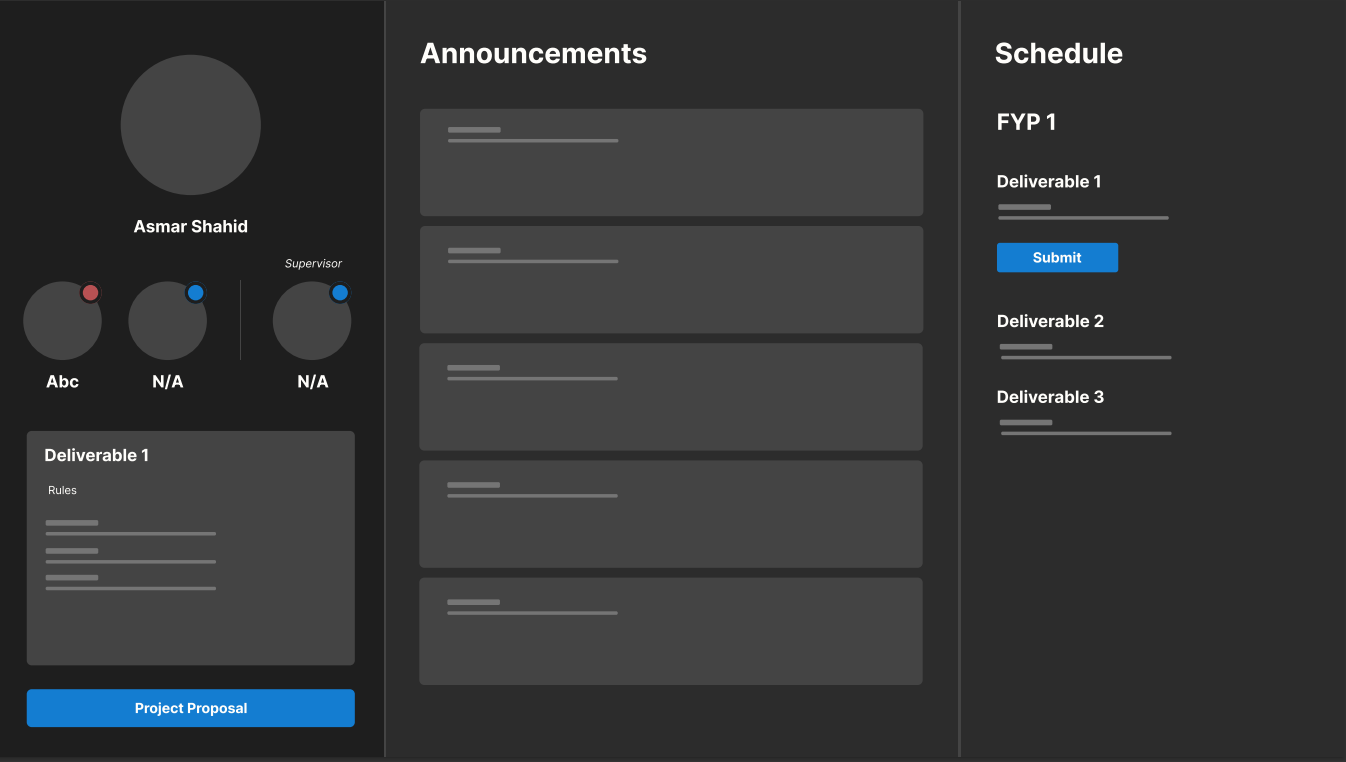
\includegraphics[width=\textwidth]{Figures/gui2}
    \caption{Dashboard Interface}
\end{figure}

\begin{figure}[H]
    \centering
    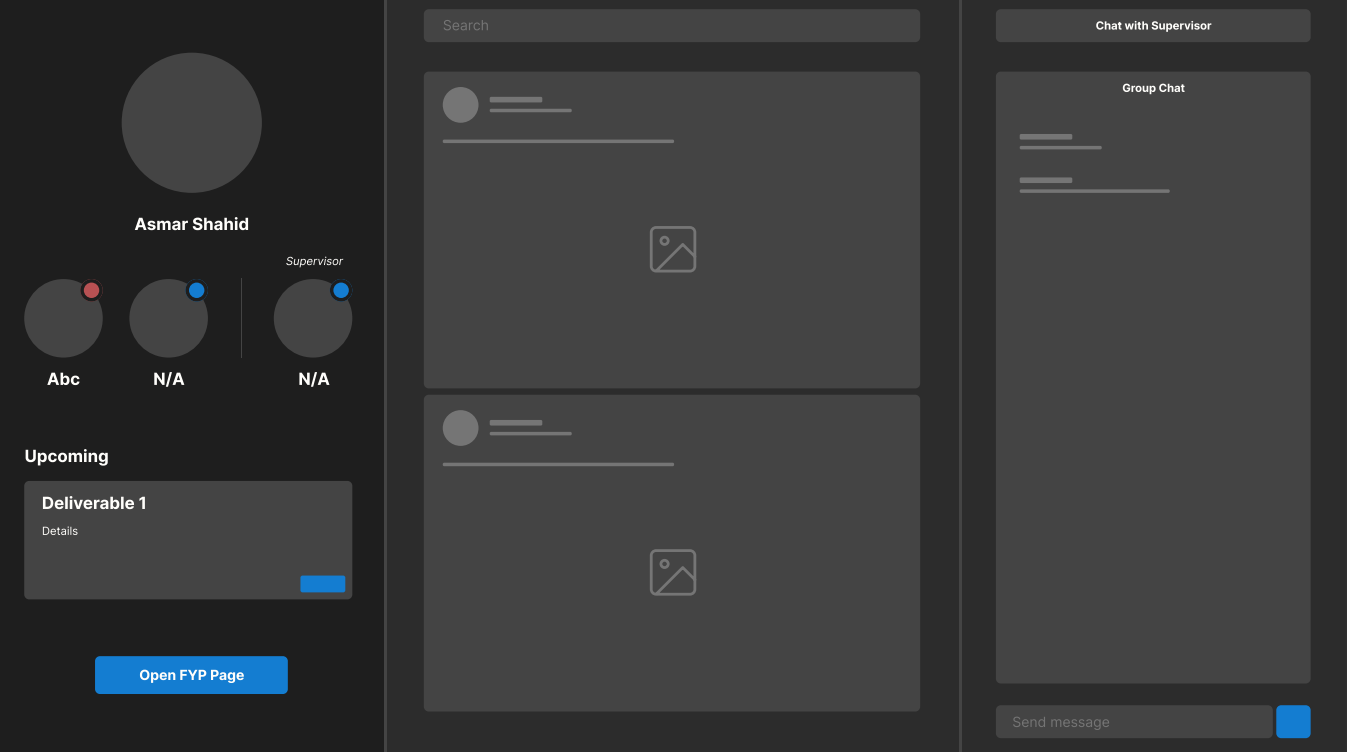
\includegraphics[width=\textwidth]{Figures/gui3}
    \caption{Post Creation Page}
\end{figure}

\begin{figure}[H]
    \centering
    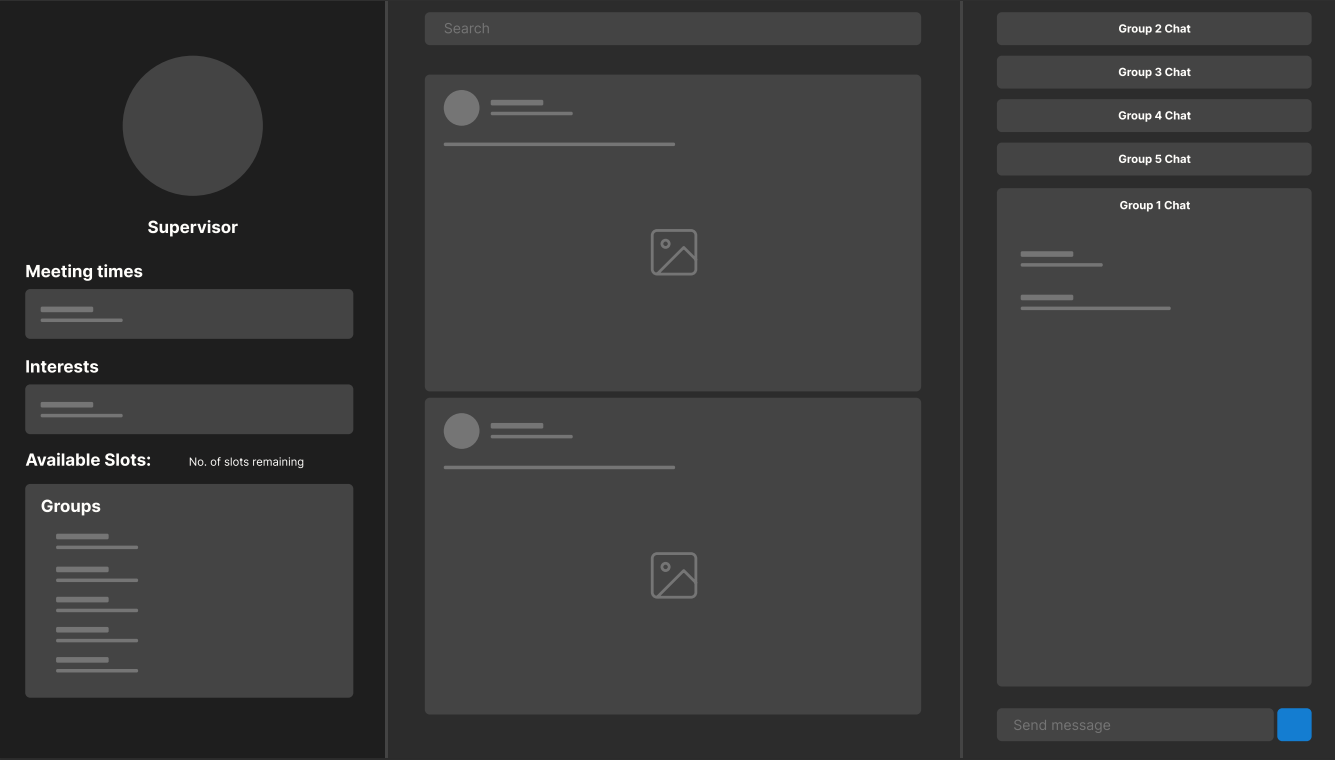
\includegraphics[width=\textwidth]{Figures/gui4}
    \caption{FYP Group Creation Interface}
\end{figure}


\pagebreak
\section{Database Design}

\subsection{ER Diagram}

\begin{figure}[H]
    \centering
    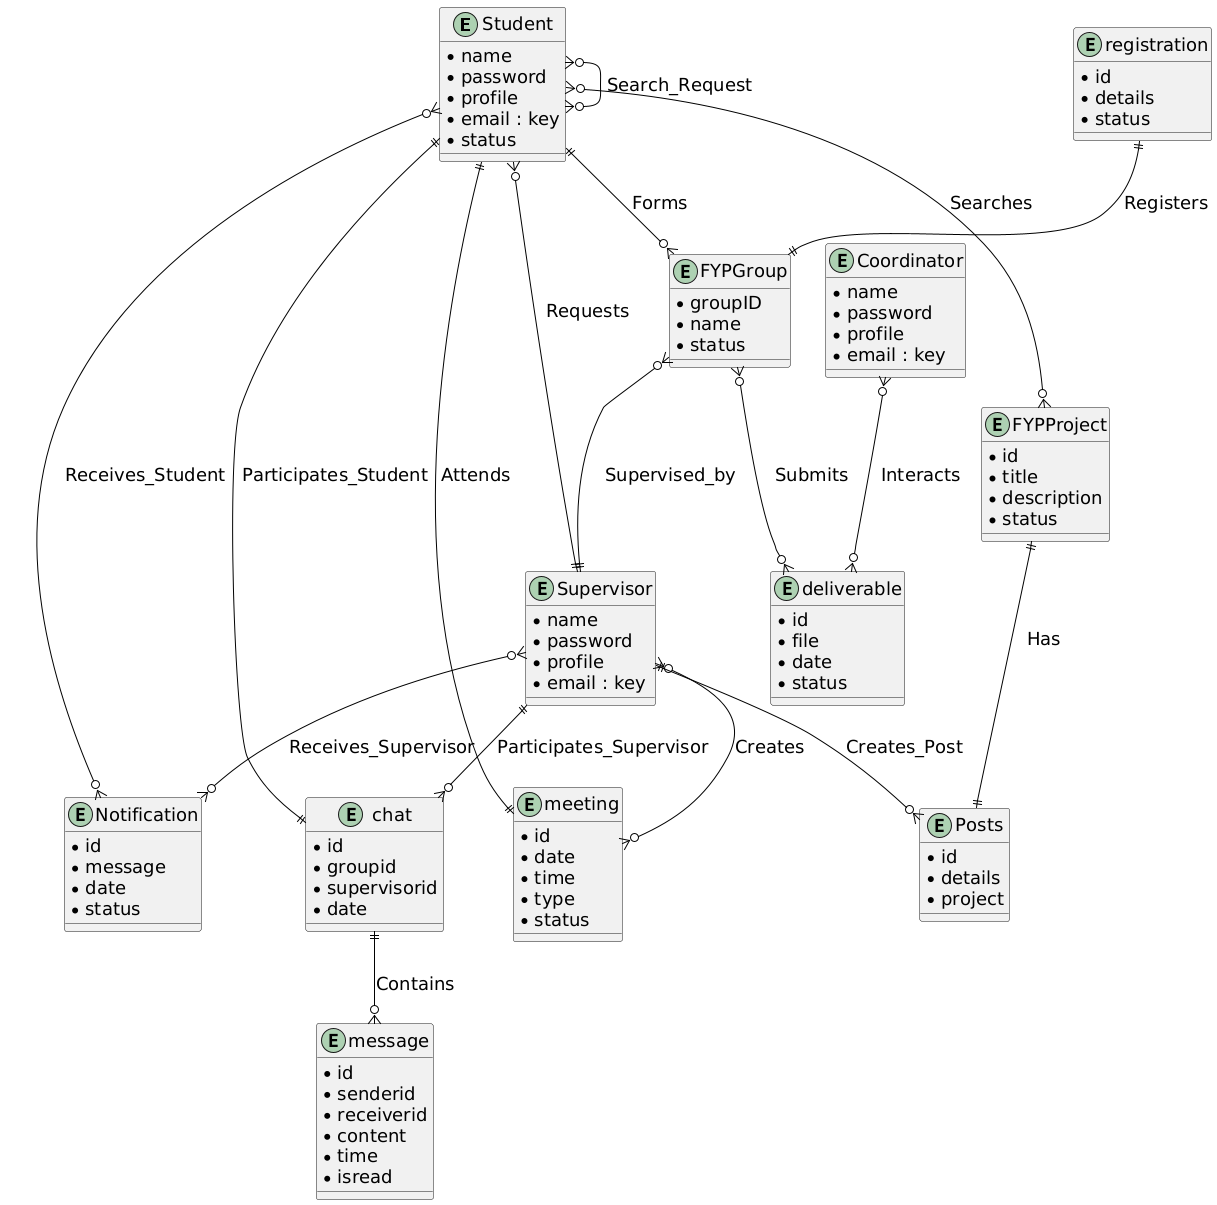
\includegraphics[width=\textwidth]{Figures/ER}
    \caption{Entity Relationship Diagram}
\end{figure}

\pagebreak
\subsection{Data Dictionary}

\begin{longtable}{|l|l|l|l|l|l|l|}
\caption{Data Dictionary} \label{tab:Data Dictionary}
\hline
\textbf{Entity} & \textbf{Attribute} & \textbf{Data Type} & \textbf{Nullable} & \textbf{Relation To} & \textbf{Relation Type} & \textbf{Description} \\ 
\hline
\endfirsthead

\hline
\textbf{Entity} & \textbf{Attribute} & \textbf{Data Type} & \textbf{Nullable} & \textbf{Relation To} & \textbf{Relation Type} & \textbf{Description} \\ 
\hline
\endhead

\hline
\multicolumn{7}{r}{\textit{Continued on the next page}} \\ 
\hline
\endfoot

\hline
\endlastfoot

Student & ID & String & No & {\begin{tabular}[c]{@{}l@{}}Supervisor, \\ FYP Group, \\ FYP Project, \\ Meeting, Chat, \\ Notification \end{tabular}} & {\begin{tabular}[c]{@{}l@{}}Many to One, \\ Many to Many, \\ Many to One, \\ Many to One, \\ Many to Many \end{tabular}} & Primary key \\ 
\hline
& Name & String & No & - & - & Full Name \\ 
\hline
& Email & String & No & - & - & Email ID \\ 
\hline
& Status & Boolean & No & - & - & Status \\ 
\hline
& Profile & Object & No & - & - & Profile Info \\ 
\hline
& Password & String & No & - & - & Password \\ 
\hline
Supervisor & ID & String & No & {\begin{tabular}[c]{@{}l@{}}Student, \\ FYP Group, \\ Meeting, \\ Notification, \\ Chat, \\ Posts \end{tabular}}  & {\begin{tabular}[c]{@{}l@{}}One to Many, \\ One to Many, \\ One to Many, \\ Many to Many, \\ One to Many, \\ One to Many \end{tabular}} & Primary key \\ 
\hline
& Name & String & No & - & - & Full Name \\ 
\hline
& Email & String & No & - & - & Email ID \\ 
\hline
& Password & String & No & - & - & Password \\ 
\hline
& Profile & Object & No & - & - & Profile Info \\ 
\hline
& Slots & int & Yes & - & - & Slots \\ 
\hline
Coordinator & ID & String & No & Deliverable & Many to Many & Primary key \\ 
\hline
& Name & String & No & - & - & Full Name \\ 
\hline
& Password & String & No & - & - & Password \\ 
\hline
& Email & String & No & - & - & Email ID \\ 
\hline
FYP Group & ID & String & No & {\begin{tabular}[c]{@{}l@{}}Student, \\ Supervisor, \\ Registration, \\ Deliverable \end{tabular}}  & {\begin{tabular}[c]{@{}l@{}} One to Many, \\ Many to One, \\ One to One, \\ One to Many \end{tabular}} & Primary key \\ 
\hline
& Name & String & No & - & - & Group Name \\ 
\hline
& Status & Boolean & No & - & - & Status \\ 
\hline
FYP Project & ID & String & No & {\begin{tabular}[c]{@{}l@{}}Student, \\ Posts \end{tabular}} & {\begin{tabular}[c]{@{}l@{}}Many to Many, \\ One to One \end{tabular}} & Primary key \\ 
\hline
& Title & String & No & - & - & Project Title \\ 
\hline
& Description & Object & No & - & - & {\begin{tabular}[c]{@{}l@{}}Project \\ Description \end{tabular}} \\ 
\hline
& Status & Boolean & No & - & - & Status \\ 
\hline
Registration & ID & String & No & FYP Group & One to One & Primary key \\ 
\hline
& Details & Object & No & - & - & {\begin{tabular}[c]{@{}l@{}}Registration \\ Details \end{tabular}} \\ 
\hline
& Status & Boolean & No & - & - & {\begin{tabular}[c]{@{}l@{}}Registration \\ Status \end{tabular}} \\ 
\hline
Deliverable & ID & String & No & {\begin{tabular}[c]{@{}l@{}}FYP Group, \\ Coordinator \end{tabular}}  & {\begin{tabular}[c]{@{}l@{}}Many to One, \\ Many to Many \end{tabular}}  & Primary key \\ 
\hline
& File & Pdf & No & - & - & {\begin{tabular}[c]{@{}l@{}}Deliverable \\ File \end{tabular}} \\ 
\hline
& Date & Date & No & - & - & {\begin{tabular}[c]{@{}l@{}}Submission \\ Date \end{tabular}} \\ 
\hline
& Status & Boolean & No & - & - & {\begin{tabular}[c]{@{}l@{}}Deliverable \\ Status \end{tabular}} \\ 
\hline
Chat & ID & String & No & {\begin{tabular}[c]{@{}l@{}}Student, \\ Supervisor, \\ Message \end{tabular}}  & {\begin{tabular}[c]{@{}l@{}}One to Many, \\ Many to One, \\ One to Many \end{tabular}}  & Primary key \\ 
\hline
& Group ID & Object & No & - & - & Group ID \\ 
\hline
& Supervisor ID & Object & No & - & - & Supervisor ID \\ 
\hline
& Date & Date & Yes & - & - & Chat Date \\ 
\hline
Message & ID & String & No & {\begin{tabular}[c]{@{}l@{}}Chat, \\ Student \end{tabular}}  & {\begin{tabular}[c]{@{}l@{}}Many to One, \\ Many to One \end{tabular}}  & Primary key \\ 
\hline
& Sender ID & Object & No & - & - & Sender ID \\ 
\hline
& Receiver ID & Object & No & - & - & Receiver ID \\ 
\hline
& Content & String & No & - & - & {\begin{tabular}[c]{@{}l@{}}Message \\ Content \end{tabular}} \\ 
\hline
& Time & Time & No & - & - & {\begin{tabular}[c]{@{}l@{}}Message \\ Time \end{tabular}} \\ 
\hline
& Read Status & Boolean & No & - & - & Read Status \\ 
\hline
Notification & ID & String & No & {\begin{tabular}[c]{@{}l@{}}Student, \\ Supervisor \end{tabular}}  & {\begin{tabular}[c]{@{}l@{}}Many to Many, \\ Many to Many \end{tabular}}  & Primary key \\ 
\hline
& Content & String & No & - & - & {\begin{tabular}[c]{@{}l@{}}Notification \\ Content \end{tabular}} \\ 
\hline
& Date & Date & No & - & - & {\begin{tabular}[c]{@{}l@{}}Notification \\ Date \end{tabular}} \\ 
\hline
& Status & Boolean & No & - & - & {\begin{tabular}[c]{@{}l@{}}Notification \\ Read Status \end{tabular}} \\ 
\hline
Posts & ID & String & No & {\begin{tabular}[c]{@{}l@{}}Supervisor, \\ FYP Project \end{tabular}}  & {\begin{tabular}[c]{@{}l@{}}Many to One, \\ One to One \end{tabular}}  & Primary key \\ 
\hline
& Details & String & No & - & - & Post Text \\ 
\hline
& Project & Object & Yes & - & - & {\begin{tabular}[c]{@{}l@{}}Linked \\ Project \end{tabular}} \\ 
\hline
Meeting & ID & String & No & {\begin{tabular}[c]{@{}l@{}}Student, \\ Supervisor \end{tabular}}  & {\begin{tabular}[c]{@{}l@{}}One to Many, \\ Many to One \end{tabular}}  & Primary key \\ 
\hline
& Time & Time & No & - & - & {\begin{tabular}[c]{@{}l@{}}Meeting \\ Time \end{tabular}} \\ 
\hline
& Date & Date & No & - & - & {\begin{tabular}[c]{@{}l@{}}Meeting \\ Date \end{tabular}} \\ 
\hline
& Type & String & Yes & - & - & {\begin{tabular}[c]{@{}l@{}}Meeting \\ Type \end{tabular}} \\ 
\hline
& Status & Boolean & No & - & - & {\begin{tabular}[c]{@{}l@{}}Meeting \\ Status \end{tabular}} \\ 
\hline

\end{longtable}



\section{Risk Analysis}
Risk analysis is an important part of the project to identify factors or risks that may adversely affect the design, implementation, and success of the FASTGlide web application. Below details the main risks that have been pinpointed in the project, their potential effects, and ways to control them:

\subsection{Data Security Risks}
\begin{itemize}
    \item The web application contains sensitive data such as students’ details, supervisors’ information, and even the final project submissions. Any compromise to this data could lead to information abuse and violations of rights.
    \item A data breach could also lead to the loss of users’ confidence and result in administrative and legal consequences for the university.
\end{itemize}
\textbf{Mitigation:}
\begin{itemize}
    \item Use high-level encryption programming for data transmission processes (HTTPS) and incorporate JSON Web Tokens (JWT) for secure login.
    \item Implement Role-Based Access Control (RBAC) to restrict access based on user categories (e.g., Students, Supervisors, Coordinators).
\end{itemize}

\subsection{System Downtime or Performance Issues}
\begin{itemize}
    \item As the number of users increases, especially during peak times (e.g., final submission deadlines), the system may experience slowdowns or downtime, affecting usability.
    \item If the system goes down during critical times, such as the final project submission period, it could lead to frustration and missed deadlines.
\end{itemize}
\textbf{Mitigation:}
\begin{itemize}
    \item Use performance optimization techniques, such as caching and asynchronous processing, to handle high loads.
\end{itemize}

\subsection{File Format and Submission Issues}
\begin{itemize}
    \item Students may occasionally fail to submit valid files, or the files may contain bugs that would impair the web application's core function of validating the format of LaTeX project deliverables.
    \item Failure to correctly validate the format may result in confusion among stakeholders and delays in project approval.
\end{itemize}
\textbf{Mitigation:}
\begin{itemize}
    \item Conduct a thorough testing process of the LaTeX format validation component to ensure the system can effectively detect and flag invalid files.
    \item Educate students on the requirements for presenting LaTeX deliverables by providing guidance on what is expected and how to format their outputs.
    \item Offer a “test submission” option for students to verify the formats and composition of their files before final submission.
\end{itemize}

\subsection{Integration with University Systems}
\begin{itemize}
    \item Since FASTGlide lacks the ability to query the university's internal databases and systems, issues may arise during integration into the existing network infrastructure, particularly for authentication or communication.
    \item The dependency on university email for authentication may pose risks if seamless integration is not achieved, or if there are prolonged downtimes of email systems.
\end{itemize}
\textbf{Mitigation:}
\begin{itemize}
    \item Implement a robust and independent authentication method using university email addresses, such as through OAuth.
    \item Design the system with contingency measures to address scenarios where email verification fails or login processes encounter issues.
\end{itemize}

\section{Conclusion}
The SRS chapter has discussed the main features and the other defining characteristics of the FASTGlide system, which facilitates the Final Year Project (FYP) for students, supervisors and coordinators. The functional requirements specify that the users will be able to use the modules of the system starting from the registration of FYP, completing the communication and submitting the deliverables which is comprehensive and user friendly. Non-functional requirements, such as performance, scalability, security, and maintainability envision that the system will continue to function well as well as work as intended in the beginning even as time progresses and the number of users increases. All in all, the thorough requirements in this chapter form the basic structure that helps attain the development and the operationalization of the FASTGlide system.

\chapter{High-Level and Low-Level Design}
This chapter discusses both the high-level and low-level design of FASTGlide, a web-based 
application aimed at solving the major problem that students face during their FYP process. In this 
section we will explore different stages involved in the achieving the desired functionality of the 
application by discussing key design decisions, strategies and tactics.
\section{System Overview}
FASTGlide is a web application, which is developed to ease the FYP (Final Year Project) process for students, supervisors, and coordinators as well. It allows students to look out for an FYP group members, find supervisors, register their projects and finally submit final report. The application helps interact all group members with their supervisors, schedule a meeting (online or physical), and send notifications and requests about project initiatives. In addition, supervisors can share projects, approve group requests, and review submitted works, and coordinators can control how the submissions are made. The application is designed in a way that all future growth targets are reached providing a good flow of use in all components that it presents.

\section{Design Considerations}
This section describes many issues that need to be addressed or resolved before attempting to devise a complete design solution.

\subsection{Assumptions and Dependencies}
The following assumptions and dependencies associated with our web application need to be addressed:

\subsubsection{User Access to Internet}
It is assumed that all users—students, supervisors, and coordinators—will have regular access to a stable internet connection. Since the system is web-based, a reliable internet connection is essential for accessing features such as FYP registration, communication, and notifications.

\subsubsection{Basic Technological Proficiency}
We assume that users will possess basic skills in using computers and the internet. This foundational knowledge will enable them to navigate the system effectively and utilize features like scheduling meetings and communicating with others.

\subsubsection{Use of University Email}
We assume that all users will have active FAST email accounts, which will be utilized for user authentication and communication through the platform. This integration ensures that users can log in with their university credentials and receive notifications and updates related to their FYP activities.

\subsubsection{Availability of Mobile Devices}
We assume that many users may access the system through their mobile devices. Therefore, the app will be designed to be mobile-friendly, ensuring it works effectively on various screen sizes.

\subsubsection{Meeting Platforms}
The system facilitates both online and physical meetings between students and supervisors. For online meetings, it assumes users can integrate commonly used platforms like Zoom, Microsoft Teams, or Google Meet. These platforms should be accessible to users for scheduling and conducting meetings effectively.

\subsubsection{Browser Compatibility}
The app assumes that users will be accessing it through standard web browsers such as Chrome, Firefox, or Safari. Ensuring compatibility across major browsers is crucial for delivering a consistent user experience.

\subsubsection{Possible and/or Probable Changes in Functionality}
The FYP process may change over time, with changes in university requirements or submission procedures. Therefore, the application is designed to be flexible and adaptable to accommodate future changes in the FYP structure or university guidelines.

\subsection{General Constraints}
\subsubsection{Internet Dependency}
A continuous and stable internet connection is required for smooth operation of the application without encountering disruptions that may hinder functionality.

\subsubsection{Device Compatibility}
Device compatibility is necessary for allowing users to have a good experience instead of restricting them to a single device. Therefore, it must function smoothly across different devices such as desktops, laptops, tablets, and smartphones.

\subsubsection{Browser Compatibility}
In addition to device compatibility, the app should also be browser-compatible for a consistent user experience. It should support major browsers such as Chrome, Firefox, and Safari.

\subsubsection{User Proficiency}
Users are assumed to have basic technological skills, which may limit functionality if users are unfamiliar with web applications.

\subsubsection{Email Requirements}
All users must have valid university email accounts for authentication, which could restrict access for those lacking such accounts.

\subsubsection{Data Integrity}
The system must maintain accurate and up-to-date information regarding users, FYP projects, and deliverable submissions to prevent errors and confusion.

\subsubsection{Institutional Policies}
The web app must comply with the university's policies regarding student data privacy, project submission guidelines, and academic integrity.

\subsubsection{Load Handling}
The web app should be able to handle peak loads during critical times such as registration periods without significant slowdowns or outages.


\subsection{Goals and Guidelines}
When designing FASTGlide, the main goal is to make the FYP process smoother and more 
manageable for everyone involved—students, supervisors, and coordinators. The system should be 
intuitive and easy to use, so that users can quickly navigate and engage with its features without 
confusion. Flexibility and scalability of the platform in addition to its intended use should also be taken into consideration. Future growth may change how university policies or guidelines affect high usage times during activities such as when project registration or submission deadlines are in place. In this domain of sensitive information pertaining to the student and project, importance of the security of the system also is a higher priority. Lastly, FASTGlide will be designed to work well on any device meaning a responsive application, whether it’s a laptop or smartphone, ensuring students can access it anytime, anywhere, without unnecessary barriers.

\subsection{Development Methods}
The project shall be managed by adopting the Scrum methodology. The Scrum project management method is very self-explanatory and flexible. Scrum utilizes short periods of time called sprints with the aim of producing working software through frequent evaluation and modification. A sprint meeting is held every day, focusing on the work that is needed to be completed on that particular day. Additionally, there is a meeting at the end of every sprint to review the work done in that incremental stage of the sprint. Furthermore, a sprint retrospective meeting is carried out before the start of the new sprint to understand what goals or other improvements need to be accomplished in the next sprint.

\section{System Architecture}

\begin{figure}[!h]
    \centering
    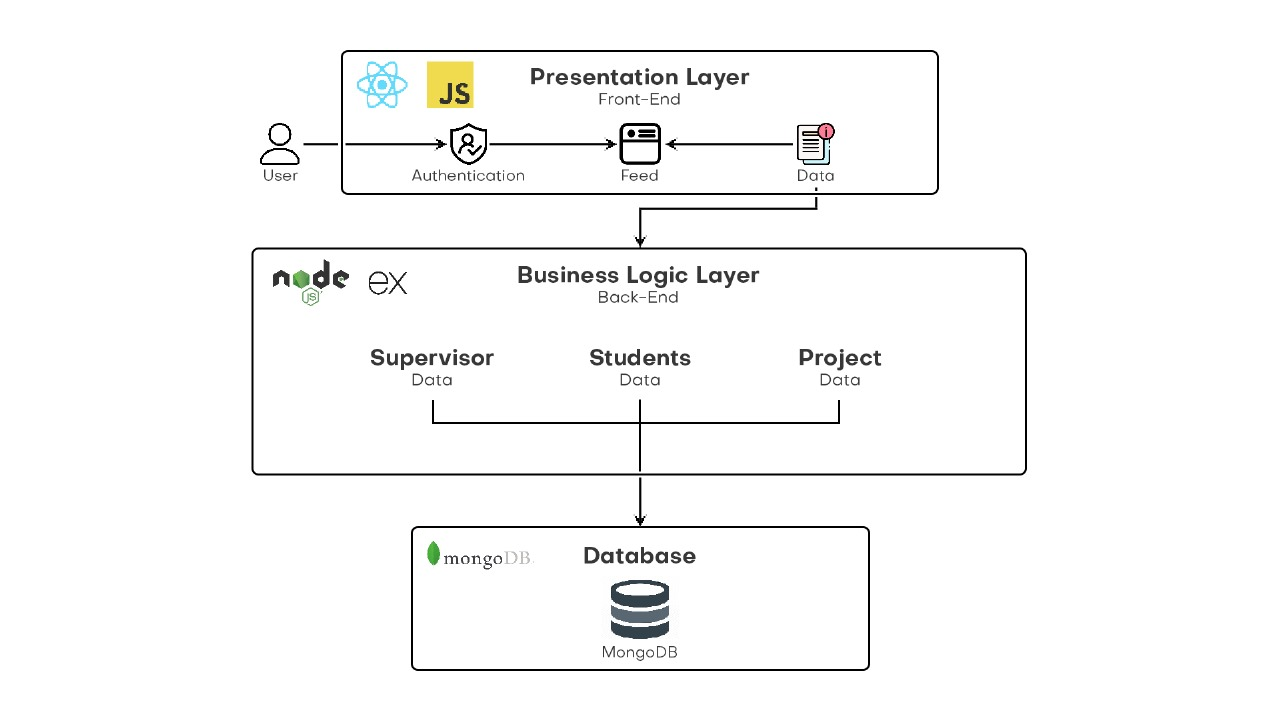
\includegraphics[width=\textwidth]{Figures/Arch}
    \caption{High-Level System Architecture Diagram}
\end{figure}

This section discusses the architecture of our system. The FASTGlide web app is designed using a layered architecture that incorporates client-server architecture. Each layer has a defined role and interacts with other layers to ensure the smooth workflow of our web app's functionality. 

The architecture is divided into three main layers:

\textbf{1. Presentation Layer (Front-End):} This layer is built using React and JavaScript, handling the user interface and rendering the app’s UI components such as authentication forms, login, user feeds, format checking, communication components, and submission components. Users interact with the system through this layer, performing actions like logging in, searching for FYP groups and supervisors, communicating, checking formats, and submitting deliverables. The Presentation Layer communicates with the backend through API calls to facilitate data operations.

\textbf{2. Business Logic Layer (Back-End):} Utilizing Node.js and Express.js, this layer manages data processing and user requests, including authentication, communication between students and supervisors, FYP registration, scheduling, and format verification of deliverables. It consists of modules for managing supervisor data, student data, FYP project data, registration data, and submissions, ensuring proper handling of user interactions and secure, efficient data processing. For format checking, the backend processes the LaTeX files of deliverables to ensure compliance with the university's formatting guidelines (e.g., margins, font size, section structure, image captions, proper hierarchy). Node.js handles this through libraries or custom scripts that parse LaTeX documents and validate their structure.

\textbf{3. Database Layer:} The system employs a NoSQL database, specifically MongoDB, responsible for storing all web app data, including student profiles, supervisor information, FYP project details, communication logs, and deliverables. MongoDB’s flexible document structure allows for easy scaling as the amount of data grows, making it suitable for storing complex, interconnected data like FYP projects and group collaborations.

By integrating these layers, FASTGlide provides a seamless and efficient experience for users while ensuring data integrity and adherence to university guidelines.


\subsection{Subsystem Architecture}
Each of the system’s layers contains subsystems that interact with one another to fulfill the system’s functionalities. The main subsystems include:

\subsubsection{Authentication Subsystem}
The Authentication Subsystem is responsible for managing user logins using university email accounts.
It ensures secure access to the platform through token-based authentication methods, likely utilizing JWT (JSON Web Tokens).
This subsystem also handles user registration and password recovery processes, enhancing user management and security.

\subsubsection{Student, Supervisor, and Project Data Subsystem}
This subsystem manages data related to students, supervisors, and FYP projects, facilitating CRUD (Create, Read, Update, Delete) operations on user and project details.
It ensures data consistency across the different user types and their associated projects, minimizing errors and ensuring accurate data representation.
Additionally, it manages relationships between users and their respective projects, ensuring that information is accessible and organized.

\subsubsection{Notification and Communication Subsystem}
The Notification and Communication Subsystem is responsible for sending notifications to students and supervisors about project updates, meeting requests, and registration statuses.
It manages communication between students and their group members, as well as interactions between students and supervisors, facilitating chat-like conversations and meeting scheduling.
This subsystem also logs communication history, providing users with an easily accessible record of interactions.

\subsubsection{Deliverable Submission and Format Subsystem}
This subsystem allows students to submit their final project deliverables for review and checks for format verification against established guidelines.
It facilitates the submission process by sending these files to coordinators and providing real-time feedback to students if submissions fail to meet the criteria.
This proactive feedback mechanism helps students correct errors before final submission, improving the quality of deliverables.

\subsubsection{File Upload and Processing Workflow}
The File Upload and Processing Workflow is designed to efficiently handle LaTeX documents, ensuring they are properly converted or compiled as needed for format verification.
This workflow includes the steps of uploading the file to the server, parsing it, and running validation checks to ensure compliance with formatting guidelines.
By addressing LaTeX format-specific issues on the back-end, the architecture ensures a thorough, scalable, and flexible validation process that can accommodate future changes to formatting standards.



\section{Architecture Strategies}
The design of the FYP Management App follows several key strategies to ensure scalability, maintainability, and user satisfaction.

\subsection{Modularity}
The architecture is organized into three distinct layers: presentation, business logic, and database. 
This division promotes modularity, enabling easier maintenance and scalability of the application. 
Each layer can be developed, tested, and deployed independently, which enhances collaboration among development teams.

\subsection{RESTful API Design}
The application utilizes a RESTful API approach for communication between the front-end and back-end.
This design ensures that data requests and responses are handled in a structured manner, which simplifies both development and troubleshooting processes.
It adheres to standard HTTP methods (GET, POST, PUT, DELETE), promoting a clear and predictable interface for developers.

\subsection{Responsive UI}
The front-end is designed to be responsive, ensuring the application functions smoothly across a variety of devices, including desktop PCs and smartphones.
This responsiveness enhances usability and accessibility, allowing users to engage with the system seamlessly, regardless of their device.
Techniques such as fluid grids, flexible images, and CSS media queries are employed to achieve a dynamic layout.

\subsection{Scalability}
MongoDB, a NoSQL database, has been selected for its flexibility and scalability.
It can efficiently handle increased data loads as the number of users (students, supervisors, and projects) grows without performance degradation.
The schema-less nature of MongoDB allows for easy modifications to the database structure, facilitating future changes and additions to the system.

\subsection{Security}
The architecture incorporates best practices for security, particularly in user authentication and data protection.
Secure token mechanisms (such as JWT) are used for authentication, ensuring that user sessions are handled securely.
Communication between different layers is protected using HTTPS protocols, and sensitive data stored in the database is encrypted to prevent unauthorized access.

\subsection{Agile Development}
The system architecture supports agile development methodologies, allowing for incremental improvements based on user feedback.
This approach fosters a flexible development process, enabling quick adaptations to changing user needs without necessitating extensive rewrites or major structural changes.
Regular sprint reviews and retrospectives help the team identify areas for enhancement and streamline future development efforts.



\section{Domain Model/Class Diagram}
\begin{figure}[!h]
    \centering
    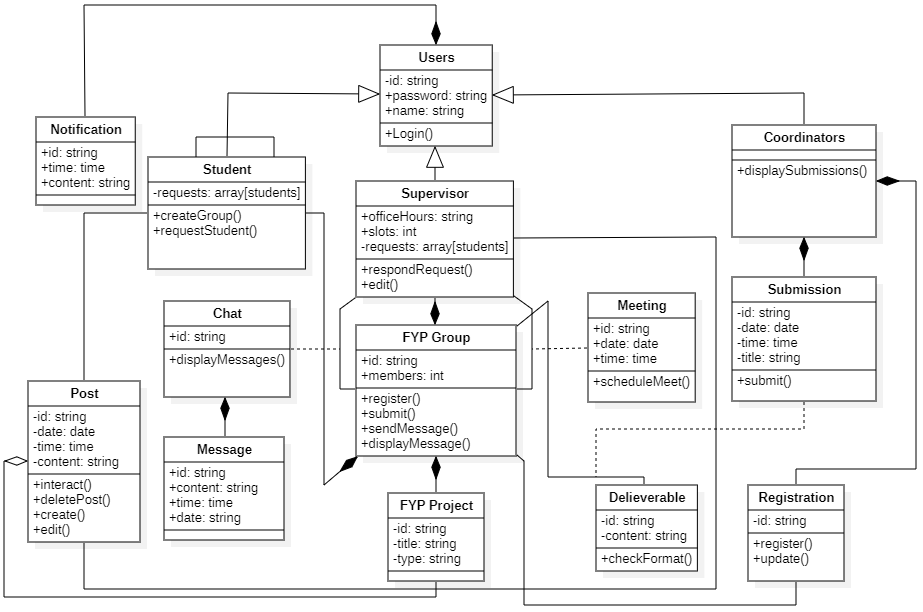
\includegraphics[width=\textwidth]{Figures/updatedClass}
    \caption{Class Diagram}
\end{figure}

\section{Policies and Tactics}
The design and development of the FASTGlide web app follows the following policies and tactics.

\subsection{Security Policy}
Given the nature of the web application, which revolves around sensitive student and faculty information, security is of utmost importance.
Communication between the client and the server is secured over HTTPS, ensuring that data is always encrypted during transmission.
For user authentication, we will implement JWT (JSON Web Tokens), a widely accepted paradigm that restricts system resources to authenticated users.
Role-based access control (RBAC) will be utilized to veil resources stored in the database, allowing only certain user roles to access their respective information. This helps maintain the integrity and confidentiality of user data.

\subsection{Performance Optimization Tactics}
The application is designed to maintain a high level of usability, even with an increasing number of users.
To achieve this, the server employs asynchronous execution and caching techniques to reduce server workload and improve response speed.
Specific features, such as LaTeX file submissions for deliverables, are optimized to handle simultaneous user interactions, ensuring that the system remains responsive even during heavy transactions.

\subsection{Tools}
FASTGlide utilizes various tools to facilitate the development process and enhance the quality of the final deliverable.
For frontend design, ReactJS libraries are employed to create an interactive user interface. The component-based structure of ReactJS promotes code reusability and maintainability, making the application easier to develop and manage over time.
On the backend, Node.js and Express.js are used to build a high-performance, scalable server.
To address storage needs, we utilize the document-oriented database, MongoDB, which is well-suited for the evolving nature of our data, including student, supervisor, and project information.
Throughout the development process, Visual Studio Code IDE is employed as the main software for code writing and management, enhancing workflow with its fast performance and rich features.

\subsection{Development Tactics}
The development process is organized into sprints according to the Scrum methodology, allowing for incremental implementation of functionality.
Development is continuously monitored through frequent sprint reviews and retrospectives, ensuring that the project remains on track and that any problems or obstacles are addressed promptly.
This agile approach fosters collaboration and adaptability, enabling the team to incorporate user feedback and adjust project priorities as needed.

\section{Conclusion}
This section provides a thorough architectural framework for the construction of the FASTGlide system. The design employs a layered architecture with three levels, namely: presentation, business logic and database, which enhances modularity, scalability and maintainability of the components. The hight level design describes structure of the entire system allowing users to interact with the platform seamlessly and it narrows down into the low level how the detailed components ,subsystems and data runs. This particular architecture gives the basis of the key functions of the FYP management system, that is, communication between students and supervisors, submissions of deliverables, and progress of students but at the same time leaves room for future developments and additional features. The design discussed in this chapter provides a sound technical base which makes the system potential and effective during its operations.


\chapter{Implementation and Test Cases}
This section talks about the development and implementation details of our FASTGlide modules.It mentions different stratgies and techniques used to implement the feature of our web app.

\section{Implementation}
The implement details of our modules are given below.

\subsection{Authentication module}
The Authentication module is very important part of the FASTGlide. Since FASTGlide is dedicated purely to students and teachers of FAST university only, any external access will be strictly prohibited. Additionally, safeguarding confidential information about students and their FYP projects is paramount, ensuring that no unauthorized users, including unverified students, can access the system.
The front end for the login is built using ReactJS, while the back end uses Node.js and Express for handling authentication logic. To prevent unauthorized access, the system employs JSON Web Tokens, a widely used and highly secure method of authentication. Tokens will have a short expiry time to minimize the risk of session hijacking and ensure users reauthenticate frequently.
Student and teacher credentials will be preloaded into the database in an encrypted form. Bcryptjs a javascript library for hashing will be used for passwords, ensuring they are stored securely and resistant to brute force attacks. A unique password generated by script will be sent to teachers and student through email with an alert to change the password immediately for enhancing security. The token will be securely stored in cookies, preventing client side scripts from accessing sensitive token data.

\subsection{FYP Management module}
Since the main objective of FASTGlide is to streamline the Final Year Project (FYP) process by helping students find supervisors, explore project ideas, and connect with group members. The FYP Portal allows students to search for other students who share similar interests, with filtering options to narrow down the search. Similarly, students can explore a list of supervisors in another section, where they can search by expertise, department, or availability and send requests for collaboration. The main page of the platform features a "Wall" where supervisors post project ideas, encouraging students to explore and collaborate on topics of mutual interest. For searching process, a GET request will be send to server along with search query since the return data of student and supervisor will be large, we will have to implement efficient queries and employ pagination and infinite scroll strategy to optimize the whole process. Similarly for implementing wall the infinite scroll strategy will be used.
A separate registration section allows students to easily create FYP groups by providing all necessary details required by university. Once a group is registered and linked to a supervisor, the system facilitates communication through features like group chats with the assigned supervisor and integrated meeting scheduling. These functionalities are implemented using simple POST requests to the server with the corresponding data. Upon successful validation, the server sends notifications to the respective students and the supervisor. For meetings, Google Meet can be used, as the university has a contract with Google that provides access to premium features of Google Meet.
Data related to students, supervisors, project ideas, and group details is stored in a MongoDB database, ensuring flexibility and scalability as data grows. RESTful APIs connect the front-end with the back-end, providing a seamless flow of data.

\subsection{Chat module}
The Chat module in FASTGlide enables real time communication between students and their supervisors. The Chat module is implemented using WebSockets, which provides full duplex communication channels over a single, long-lived connection. This enables real-time message exchange without the need for continuous page refreshes. A WebSocket client is integrated into the React components using a WebSocket library such as Socket.IO. When a user sends a message, it is emitted to the server, and any responses from the supervisor or group members are immediately received and displayed in the chat window. On the back end, nodejs with Socket.IO is used to handle web socket connections. The server manages multiple chat rooms, where each room corresponds to a specific FYP group or a student-supervisor conversation. When a user logs into the platform, they are connected to their relevant chat rooms based on their active groups or assigned supervisors. The web socket server listens for incoming connections, and when a message is received from a user, it is broadcast to all users in the same chat room. To ensure security, the system uses json web  token authentication for validating users before allowing them to join chat rooms. Messages sent within the chat are stored in a MongoDB database to maintain chat history.


\subsection{Latex Checking module}
The LaTeX Report Checking Module in FASTGlide is designed to ensure that student FYP submissions are according to university formatting guidelines. The module utilizes node and express to manage file uploads, and multer library to handle the extraction of ZIP archives containing LaTeX files. Once the ZIP file is extracted, the module checks the LaTeX content for several critical formatting issues, such as verifying that student names are properly listed in the required section, ensuring references in the .bib file follow the correct format, and checking that figures include captions, ensuring they do not start with "This figure...". The system also verifies that all required figures and signatures are present. Additionally, the LaTeX document is compiled using pdflatex, and if compilation fails, the log file is analyzed for errors, providing detailed feedback on the issue. The module also includes functionality to extract student names from the LaTeX content and checks for correct inclusion within specified sections. We are currently using Regex for parsing the latex file. There are libraries available as well for parsing like latex.js or TeXParser that can help break down LaTeX into a more structured representation. We will be using computer vision techniques a library such as OpenCV for detecting layout issues like incorrect spacing or margin problems in the compiled PDF along with library pdf2text to analyze the spacing and layout in a more programmatic manner. The results and findings will be sent back to client in a response body which will be displayed to user in defined UI.




\chapter{Conclusion and Future Work}

The web-based application FASTGlide is being developed to make the Final Year Project  process easy, providing a platform for students to find supervisors, form groups, and collaborate on projects. In this phase, we have focused primarily on developing the LaTeX module, which aims to automate the checking and validation of LaTeX document formats in accordance with university guidelines. This module addresses key issues faced by evaluators and coordinators who currently must manually check each student's FYP report for common formatting and structural errors. By automating this process, our module helps students identify and correct major mistakes before submission, significantly reducing the workload for evaluators and ensuring that reports adhere to university standards.
The current implementation provides and solves the basic validation issues faced for LaTeX documents, such as checking the format for student names, figure captions, and references, using regex and simple parsing techniques. However, this phase has been limited to addressing the most common issues, and we plan to extend the module’s capabilities in future phases. The next step will include more rigorous and strict checking mechanisms, ensuring that the LaTeX file complies fully with university guidelines, such as proper spacing, consistent formatting, and accurate citation styles. This will involve integrating advanced LaTeX parsing libraries and employing image processing tools to check for spacing and layout errors, further improving the accuracy and comprehensiveness of the validation.
Looking ahead, the FYP-2 phase will focus on completing the remaining functional requirements of the system, including the FYP management module, chat module and authentication module. Additionally, the LaTeX checking module will be enhanced to provide more detailed feedback and automatic correction suggestions for students, enabling a smoother and more efficient submission process. Testing and refinement will be conducted to ensure the system is scalable, robust, and user-friendly.
In conclusion, the work completed so far lays a solid foundation for FASTGlide. The LaTeX module addresses critical pain points faced by evaluators and students by automating the document validation process, helping students avoid major errors before submission. Future work will focus on improving the more in depth checking of LaTeX files, aligning them more closely with university guidelines, and further enhancing the system’s overall functionality. This will bring us closer to delivering a comprehensive and efficient solution for FYP management and evaluation.



{
\bibliographystyle{ieeetr}
\bibliography{fypbib} %specify your .bib file here
}


\end{document}


